%%
%% Automatically generated ptex2tex (extended LaTeX) file
%% from Doconce source
%% http://code.google.com/p/doconce/
%%

\documentclass{article}

\usepackage{relsize,epsfig,makeidx,amsmath,amsfonts}
\usepackage[latin1]{inputenc}
\usepackage{ptex2tex,subfigure}
\usepackage{minted}  % requires latex -shell-escape (for Minted_* ptex2tex envirs)


\usepackage[%
colorlinks=true,
linkcolor=blue,
citecolor=black,
filecolor=blue,
urlcolor=blue]{hyperref}
%\hyperbaseurl{}   % hyperlinks are relative to this root

\newcommand{\inlinecomment}[2]{  ({\bf #1}: \emph{#2})  }
%\newcommand{\inlinecomment}[2]{}  % turn off inline comments

\makeindex

\begin{document}

\newcommand{\beqa}{\begin{eqnarray}}
\newcommand{\eeqa}{\end{eqnarray}}
\newcommand{\ep}{\thinspace . }
\newcommand{\uvec}{\vec u}
\newcommand{\mathbfx}[1]{{\mbox{\boldmath $#1$}}}
\newcommand{\Q}{\mathbfx{Q}}

\newcommand{\x}{\mathbfx{x}}
\newcommand{\normalvec}{\mathbfx{n}}
\newcommand{Ddt}[1]{\frac{D#1}{dt}}




% ----------------- Title -------------------------

\begin{center}
{\LARGE\bf Doconce Description}
\end{center}




% ----------------- Author(s) -------------------------

\begin{center}
{\bf Hans Petter Langtangen${}^{1, 2}$} \\ [0mm]
\end{center}

\begin{center}
% List of all institutions:
\centerline{{\small ${}^1$Simula Research Laboratory}}
\centerline{{\small ${}^2$University of Oslo}}
\end{center}
% ----------------- End of author(s) -------------------------



% ----------------- Date -------------------------


\begin{center}
Jun 24, 2012
\end{center}


% lines beginning with # are comment lines


\section{What Is Doconce?}

\label{what:is:doconce}
\index{doconce!short explanation}

Doconce is two things:

\begin{enumerate}
 \item Doconce is a very simple and minimally tagged markup language that
    looks like ordinary ASCII text (much like what you would use in an
    email), but the text can be transformed to numerous other formats,
    including HTML, Pandoc, Google wiki, {\LaTeX}, PDF, reStructuredText
    (reST), Sphinx, Epytext, and also plain text (where non-obvious
    formatting/tags are removed for clear reading in, e.g.,
    emails). From reST you can (via {\fontsize{10pt}{10pt}\verb!rst2*!} programs) go to XML, HTML,
    {\LaTeX}, PDF, OpenOffice, and from the latter (via {\fontsize{10pt}{10pt}\verb!unoconv!}) to
    RTF, numerous MS Word formats (including MS Office Open XML),
    DocBook, PDF, MediaWiki, XHTML. From Pandoc one can generate
    Markdown, reST, {\LaTeX}, HTML, PDF, DocBook XML, OpenOffice, GNU
    Texinfo, MediaWiki, RTF, Groff, and other formats.

 \item Doconce is a working strategy for never duplicating information.
    Text is written in a single place and then transformed to
    a number of different destinations of diverse type (software
    source code, manuals, tutorials, books, wikis, memos, emails, etc.).
    The Doconce markup language support this working strategy.
    The slogan is: "Write once, include anywhere".
\end{enumerate}

\noindent
Here are some Doconce features:

\begin{itemize}
  \item Doconce markup does include tags, so the format is more tagged than
    Markdown and Pandoc, but less than reST, and very much less than
    {\LaTeX} and HTML.

  \item Doconce can be converted to plain \emph{untagged} text,
    often desirable for computer programs and email.

  \item Doconce has good support for copying in parts of computer code
    directly from the source code files via regular expressions
    for the start and end lines.

  \item Doconce has full support for {\LaTeX} math and integrates well
    with big {\LaTeX} projects (books).

  \item Doconce is almost self-explanatory and is a handy starting point
    for generating documents in more complicated markup languages, such
    as Google wiki, {\LaTeX}, and Sphinx. A primary application of Doconce
    is just to make the initial versions of a Sphinx or wiki document.

  \item Contrary to the similar (and superior) Pandoc translator, Doconce
    supports Sphinx, Google wiki, Creole wiki (for bitbucket.org),
    lots of computer code environments in {\LaTeX}, and a special exercise
    syntax. Doconce also also runs preprocessors (including Mako)
    such that the author can mix ordinary text with programming
    construction for generating parts of the text.
\end{itemize}

\noindent
Doconce was particularly written for the following sample applications:

\begin{itemize}
  \item Large books written in {\LaTeX}, but where many pieces (computer demos,
    projects, examples) can be written in Doconce to appear in other
    contexts in other formats, including plain HTML, Sphinx, wiki, or MS Word.

  \item Software documentation, primarily Python doc strings, which one wants
    to appear as plain untagged text for viewing in Pydoc, as reStructuredText
    for use with Sphinx, as wiki text when publishing the software at
    web sites, and as {\LaTeX} integrated in, e.g., a thesis.

  \item Quick memos, which start as plain text in email, then some small
    amount of Doconce tagging is added, before the memos can appear as
    Sphinx web pages, MS Word documents, or in wikis.
\end{itemize}

\noindent
History: Doconce was developed in 2006 at a time when most popular
markup languages used quite some tagging.  Later, almost untagged
markup languages like Markdown and Pandoc became popular. Doconce is
not a replacement of Pandoc, which is a considerably more
sophisticated project. Moreover, Doconce was developed mainly to
fulfill the needs for a flexible source code base for books with much
mathematics and computer code.

Disclaimer: Doconce is a simple tool, largely based on interpreting
and handling text through regular expressions. The possibility for
tweaking the layout is obviously limited since the text can go to
all sorts of sophisticated markup languages. Moreover, because of
limitations of regular expressions, some formatting of Doconce syntax
may face problems when transformed to HTML, {\LaTeX}, Sphinx, and similar
formats.

\subsection{Dependencies and Installation}

Doconce itself is pure Python code hosted at \href{{http://code.google.com/p/doconce}}{\nolinkurl{http://code.google.com/p/doconce}}.  Its installation from the
Mercurial ({\fontsize{10pt}{10pt}\verb!hg!}) source follows the standard procedure:
\vspace{4pt}
\begin{Verbatim}[numbers=none,frame=lines,label=\fbox{{\tiny Terminal}},fontsize=\fontsize{9pt}{9pt},
labelposition=topline,framesep=2.5mm,framerule=0.7pt]
# Doconce
hg clone https://doconce.googlecode.com/hg/ doconce
cd doconce
sudo python setup.py install
cd ..
\end{Verbatim}

If you make use of the \href{{http://code.google.com/p/preprocess}}{Preprocess}
preprocessor, this program must be installed:
\vspace{4pt}
\begin{Verbatim}[numbers=none,frame=lines,label=\fbox{{\tiny Terminal}},fontsize=\fontsize{9pt}{9pt},
labelposition=topline,framesep=2.5mm,framerule=0.7pt]
svn checkout http://preprocess.googlecode.com/svn/trunk/ preprocess
cd preprocess
cd doconce
sudo python setup.py install
cd ..
\end{Verbatim}
A much more advanced alternative to Preprocess is
\href{{http://www.makotemplates.org}}{Mako}. Its installation is most
conveniently done by {\fontsize{10pt}{10pt}\verb!pip!},
\vspace{4pt}
\begin{Verbatim}[numbers=none,frame=lines,label=\fbox{{\tiny Terminal}},fontsize=\fontsize{9pt}{9pt},
labelposition=topline,framesep=2.5mm,framerule=0.7pt]
pip install Mako
\end{Verbatim}
This command requires {\fontsize{10pt}{10pt}\verb!pip!} to be installed. On Debian Linux systems,
such as Ubuntu, the installation is simply done by
\vspace{4pt}
\begin{Verbatim}[numbers=none,frame=lines,label=\fbox{{\tiny Terminal}},fontsize=\fontsize{9pt}{9pt},
labelposition=topline,framesep=2.5mm,framerule=0.7pt]
sudo apt-get install python-pip
\end{Verbatim}
Alternatively, one can install from the {\fontsize{10pt}{10pt}\verb!pip!} \href{{http://pypi.python.org/pypi/pip}}{source code}.

To make {\LaTeX}
documents (without going through the reStructuredText format) you
need \href{{http://code.google.com/p/ptex2tex}}{ptex2tex}, which is
installed by
\vspace{4pt}
\begin{Verbatim}[numbers=none,frame=lines,label=\fbox{{\tiny Terminal}},fontsize=\fontsize{9pt}{9pt},
labelposition=topline,framesep=2.5mm,framerule=0.7pt]
svn checkout http://ptex2tex.googlecode.com/svn/trunk/ ptex2tex
cd ptex2tex
sudo python setup.py install
cd latex
sh cp2texmf.sh  # copy stylefiles to ~/texmf directory
cd ../..
\end{Verbatim}
As seen, {\fontsize{10pt}{10pt}\verb!cp2texmf.sh!} copies some special stylefiles that
that {\fontsize{10pt}{10pt}\verb!ptex2tex!} potentially makes use of. Some more standard stylefiles
are also needed. These are installed by
\vspace{4pt}
\begin{Verbatim}[numbers=none,frame=lines,label=\fbox{{\tiny Terminal}},fontsize=\fontsize{9pt}{9pt},
labelposition=topline,framesep=2.5mm,framerule=0.7pt]
sudo apt-get install texlive-latex-extra
\end{Verbatim}
on Debian Linux (including Ubuntu) systems. TeXShop on Mac comes with
the necessary stylefiles (if not, they can be found by googling and installed
manually in the {\fontsize{10pt}{10pt}\verb!~/texmf/tex/latex/misc!} directory).

The \emph{minted} {\LaTeX} style is offered by {\fontsize{10pt}{10pt}\verb!ptex2tex!} and popular among
users. This style requires the package \href{{http://pygments.org}}{Pygments}:
\vspace{4pt}
\begin{Verbatim}[numbers=none,frame=lines,label=\fbox{{\tiny Terminal}},fontsize=\fontsize{9pt}{9pt},
labelposition=topline,framesep=2.5mm,framerule=0.7pt]
hg clone ssh://hg@bitbucket.org/birkenfeld/pygments-main pygments
cd pygments
sudo python setup.py install
\end{Verbatim}
If you use the minted style, you have to enable it by running
{\fontsize{10pt}{10pt}\verb!ptex2tex -DMINTED!} and then {\fontsize{10pt}{10pt}\verb!latex -shell-escape!}, see
the Section~\ref{doconce2formats}.

For {\fontsize{10pt}{10pt}\verb!rst!} output and further transformation to {\LaTeX}, HTML, XML,
OpenOffice, and so on, one needs \href{{http://docutils.sourceforge.net}}{docutils}.
The installation can be done by
\vspace{4pt}
\begin{Verbatim}[numbers=none,frame=lines,label=\fbox{{\tiny Terminal}},fontsize=\fontsize{9pt}{9pt},
labelposition=topline,framesep=2.5mm,framerule=0.7pt]
svn checkout http://docutils.svn.sourceforge.net/svnroot/docutils/trunk/docutils
cd docutils
sudo python setup.py install
cd ..
\end{Verbatim}
To use the OpenOffice suite you will typically on Debian systems install
\vspace{4pt}
\begin{Verbatim}[numbers=none,frame=lines,label=\fbox{{\tiny Terminal}},fontsize=\fontsize{9pt}{9pt},
labelposition=topline,framesep=2.5mm,framerule=0.7pt]
sudo apt-get install unovonv libreoffice libreoffice-dmaths
\end{Verbatim}

There is a possibility to create PDF files from reST documents
using ReportLab instead of {\LaTeX}. The enabling software is
\href{{http://code.google.com/p/rst2pdf}}{rst2pdf}. Either download the tarball
or clone the svn repository, go to the {\fontsize{10pt}{10pt}\verb!rst2pdf!} directory and
run {\fontsize{10pt}{10pt}\verb!sudo python setup.py install!}.


Output to {\fontsize{10pt}{10pt}\verb!sphinx!} requires of course \href{{http://sphinx.pocoo.org}}{Sphinx},
installed by
\vspace{4pt}
\begin{Verbatim}[numbers=none,frame=lines,label=\fbox{{\tiny Terminal}},fontsize=\fontsize{9pt}{9pt},
labelposition=topline,framesep=2.5mm,framerule=0.7pt]
hg clone https://bitbucket.org/birkenfeld/sphinx
cd sphinx
sudo python setup.py install
cd ..
\end{Verbatim}

When the output format is {\fontsize{10pt}{10pt}\verb!epydoc!} one needs that program too, installed
by
\vspace{4pt}
\begin{Verbatim}[numbers=none,frame=lines,label=\fbox{{\tiny Terminal}},fontsize=\fontsize{9pt}{9pt},
labelposition=topline,framesep=2.5mm,framerule=0.7pt]
svn co https://epydoc.svn.sourceforge.net/svnroot/epydoc/trunk/epydoc epydoc
cd epydoc
sudo make install
cd ..
\end{Verbatim}

Finally, translation to {\fontsize{10pt}{10pt}\verb!pandoc!} requires the
\href{{http://johnmacfarlane.net/pandoc/}}{Pandoc} program
(written in Haskell) to be installed.
\vspace{4pt}
\begin{Verbatim}[numbers=none,frame=lines,label=\fbox{{\tiny Terminal}},fontsize=\fontsize{9pt}{9pt},
labelposition=topline,framesep=2.5mm,framerule=0.7pt]
sudo apt-get install pandoc
\end{Verbatim}

\paragraph{Remark.}
Several of the packages above installed from source code
are also available in Debian-based system through the
{\fontsize{10pt}{10pt}\verb!apt-get install!} command. However, we recommend installation directly
from the version control system repository as there might be important
updates and bug fixes. For {\fontsize{10pt}{10pt}\verb!svn!} directories, go to the directory,
run {\fontsize{10pt}{10pt}\verb!svn update!}, and then {\fontsize{10pt}{10pt}\verb!sudo python setup.py install!}. For
Mercurial ({\fontsize{10pt}{10pt}\verb!hg!}) directories, go to the directory, run
{\fontsize{10pt}{10pt}\verb!hg pull; hg update!}, and then {\fontsize{10pt}{10pt}\verb!sudo python setup.py install!}.
Doconce itself is frequently updated so these commands should be
run regularly.


% 
% Here are some comment lines that do not affect any formatting
% these lines are converted to comments in the output format.
% This may have some side effects, especially in rst and sphinx
% where lines following the comment may be taken as part of
% the comment if there are no blank lines after the comment.
% 
% One can use ## and the mako preprocessor to remove comments
% \emph{before} doconce sees the text. That can be useful when
% doconce comments interferes with formatting.
% The mako tool also supports <%doc> .. </%doc>
% 

\subsection{Demos}

\index{demos}

The current text is generated from a Doconce format stored in the
\vspace{4pt}
\begin{Verbatim}[numbers=none,frame=lines,label=\fbox{{\tiny Terminal}},fontsize=\fontsize{9pt}{9pt},
labelposition=topline,framesep=2.5mm,framerule=0.7pt]
docs/manual/manual.do.txt
\end{Verbatim}
file in the Doconce source code tree. We have made a
\href{{https://doconce.googlecode.com/hg/doc/demos/manual/index.html}}{demo web page}
where you can compare the Doconce source with the output in many
different formats: HTML, {\LaTeX}, plain text, etc.

The file {\fontsize{10pt}{10pt}\verb!make.sh!} in the same directory as the {\fontsize{10pt}{10pt}\verb!manual.do.txt!} file
(the current text) shows how to run {\fontsize{10pt}{10pt}\verb!doconce format!} on the
Doconce file to obtain documents in various formats.

Another demo is found in
\vspace{4pt}
\begin{Verbatim}[numbers=none,frame=lines,label=\fbox{{\tiny Terminal}},fontsize=\fontsize{9pt}{9pt},
labelposition=topline,framesep=2.5mm,framerule=0.7pt]
docs/tutorial/tutorial.do.txt
\end{Verbatim}
In the {\fontsize{10pt}{10pt}\verb!tutorial!} directory there is also a {\fontsize{10pt}{10pt}\verb!make.sh!} file producing a
lot of formats, with a corresponding
\href{{https://doconce.googlecode.com/hg/doc/demos/tutorial/index.html}}{web demo}
of the results.

% Example on including another Doconce file:


\section{From Doconce to Other Formats}

\label{doconce2formats}

Transformation of a Doconce document {\fontsize{10pt}{10pt}\verb!mydoc.do.txt!} to various other
formats applies the script {\fontsize{10pt}{10pt}\verb!doconce format!}:
\vspace{4pt}
\begin{Verbatim}[numbers=none,frame=lines,label=\fbox{{\tiny Terminal}},fontsize=\fontsize{9pt}{9pt},
labelposition=topline,framesep=2.5mm,framerule=0.7pt]
Terminal> doconce format format mydoc.do.txt
\end{Verbatim}
or just
\vspace{4pt}
\begin{Verbatim}[numbers=none,frame=lines,label=\fbox{{\tiny Terminal}},fontsize=\fontsize{9pt}{9pt},
labelposition=topline,framesep=2.5mm,framerule=0.7pt]
Terminal> doconce format format mydoc
\end{Verbatim}
The {\fontsize{10pt}{10pt}\verb!mako!} or {\fontsize{10pt}{10pt}\verb!preprocess!} programs are always used to preprocess the
file first, and options to {\fontsize{10pt}{10pt}\verb!mako!} or {\fontsize{10pt}{10pt}\verb!preprocess!} can be added after the
filename. For example,
\vspace{4pt}
\begin{Verbatim}[numbers=none,frame=lines,label=\fbox{{\tiny Terminal}},fontsize=\fontsize{9pt}{9pt},
labelposition=topline,framesep=2.5mm,framerule=0.7pt]
Terminal> doconce format latex mydoc -Dextra_sections -DVAR1=5     # preprocess
Terminal> doconce format latex yourdoc extra_sections=True VAR1=5  # mako
\end{Verbatim}
The variable {\fontsize{10pt}{10pt}\verb!FORMAT!} is always defined as the current format when
running {\fontsize{10pt}{10pt}\verb!preprocess!}. That is, in the last example, {\fontsize{10pt}{10pt}\verb!FORMAT!} is
defined as {\fontsize{10pt}{10pt}\verb!latex!}. Inside the Doconce document one can then perform
format specific actions through tests like {\fontsize{10pt}{10pt}\verb!#if FORMAT == "latex"!}.

Inline comments in the text are removed from the output by
\vspace{4pt}
\begin{Verbatim}[numbers=none,frame=lines,label=\fbox{{\tiny Terminal}},fontsize=\fontsize{9pt}{9pt},
labelposition=topline,framesep=2.5mm,framerule=0.7pt]
Terminal> doconce format latex mydoc --skip_inline_comments
\end{Verbatim}
One can also remove all such comments from the original Doconce
file by running:
\begin{Verbatim}[fontsize=\fontsize{9pt}{9pt},tabsize=8,baselinestretch=0.85,
fontfamily=tt,xleftmargin=7mm]
Terminal> doconce remove_inline_comments mydoc
\end{Verbatim}
\noindent
This action is convenient when a Doconce document reaches its final form
and comments by different authors should be removed.

\subsection{HTML}

Making an HTML version of a Doconce file {\fontsize{10pt}{10pt}\verb!mydoc.do.txt!}
is performed by
\vspace{4pt}
\begin{Verbatim}[numbers=none,frame=lines,label=\fbox{{\tiny Terminal}},fontsize=\fontsize{9pt}{9pt},
labelposition=topline,framesep=2.5mm,framerule=0.7pt]
Terminal> doconce format html mydoc
\end{Verbatim}
The resulting file {\fontsize{10pt}{10pt}\verb!mydoc.html!} can be loaded into any web browser for viewing.

\subsection{Pandoc}

Output in Pandoc's extended Markdown format results from
\vspace{4pt}
\begin{Verbatim}[numbers=none,frame=lines,label=\fbox{{\tiny Terminal}},fontsize=\fontsize{9pt}{9pt},
labelposition=topline,framesep=2.5mm,framerule=0.7pt]
Terminal> doconce format pandoc mydoc
\end{Verbatim}
The name of the output file is {\fontsize{10pt}{10pt}\verb!mydoc.mkd!}.
From this format one can go to numerous other formats:
\vspace{4pt}
\begin{Verbatim}[numbers=none,frame=lines,label=\fbox{{\tiny Terminal}},fontsize=\fontsize{9pt}{9pt},
labelposition=topline,framesep=2.5mm,framerule=0.7pt]
Terminal> pandoc -R -t mediawiki -o mydoc.mwk mydoc.mkd
\end{Verbatim}
Pandoc supports {\fontsize{10pt}{10pt}\verb!latex!}, {\fontsize{10pt}{10pt}\verb!html!}, {\fontsize{10pt}{10pt}\verb!odt!} (OpenOffice), {\fontsize{10pt}{10pt}\verb!docx!} (Microsoft
Word), {\fontsize{10pt}{10pt}\verb!rtf!}, {\fontsize{10pt}{10pt}\verb!texinfo!}, to mention some. The {\fontsize{10pt}{10pt}\verb!-R!} option makes
Pandoc pass raw HTML or {\LaTeX} to the output format instead of ignoring it.
See the \href{{http://johnmacfarlane.net/pandoc/README.html}}{Pandoc documentation}
for the many features of the {\fontsize{10pt}{10pt}\verb!pandoc!} program.

Pandoc is useful to go from {\LaTeX} mathematics to, e.g., HTML or MS Word.
There are two ways (experiment to find the best one for your document):
{\fontsize{10pt}{10pt}\verb!doconce format pandoc!} and then translating using {\fontsize{10pt}{10pt}\verb!pandoc!}, or
{\fontsize{10pt}{10pt}\verb!doconce format latex!}, and then going from {\LaTeX} to the desired format
using {\fontsize{10pt}{10pt}\verb!pandoc!}.
Here is an example on the latter strategy:
\vspace{4pt}
\begin{Verbatim}[numbers=none,frame=lines,label=\fbox{{\tiny Terminal}},fontsize=\fontsize{9pt}{9pt},
labelposition=topline,framesep=2.5mm,framerule=0.7pt]
Terminal> doconce format latex mydoc
Terminal> doconce ptex2tex mydoc
Terminal> pandoc -f latex -t docx -o mydoc.docx mydoc.tex
\end{Verbatim}
When we go through {\fontsize{10pt}{10pt}\verb!pandoc!}, only single equations or {\fontsize{10pt}{10pt}\verb!align*!}
environments are well understood.

Quite some {\fontsize{10pt}{10pt}\verb!doconce replace!} and {\fontsize{10pt}{10pt}\verb!doconce subst!} edits might be needed
on the {\fontsize{10pt}{10pt}\verb!.mkd!} or {\fontsize{10pt}{10pt}\verb!.tex!} files to successfully have mathematics that is
well translated to MS Word.  Also when going to reStructuredText using
Pandoc, it can be advantageous to go via {\LaTeX}.

Here is an example where we take a Doconce snippet (without title, author,
and date), maybe with some unnumbered equations, and quickly generate
HTML with mathematics displayed my MathJax:
\vspace{4pt}
\begin{Verbatim}[numbers=none,frame=lines,label=\fbox{{\tiny Terminal}},fontsize=\fontsize{9pt}{9pt},
labelposition=topline,framesep=2.5mm,framerule=0.7pt]
Terminal> doconce format pandoc mydoc
Terminal> pandoc -t html -o mydoc.html -s --mathjax mydoc.mkd
\end{Verbatim}
The {\fontsize{10pt}{10pt}\verb!-s!} option adds a proper header and footer to the {\fontsize{10pt}{10pt}\verb!mydoc.html!} file.
This recipe is a quick way of makeing HTML notes with (some) mathematics.

\subsection{{\LaTeX}}

Making a {\LaTeX} file {\fontsize{10pt}{10pt}\verb!mydoc.tex!} from {\fontsize{10pt}{10pt}\verb!mydoc.do.txt!} is done in two steps:
% Note: putting code blocks inside a list is not successful in many
% formats - the text may be messed up. A better choice is a paragraph
% environment, as used here.

\paragraph{Step 1.}
Filter the doconce text to a pre-LaTeX form {\fontsize{10pt}{10pt}\verb!mydoc.p.tex!} for
     {\fontsize{10pt}{10pt}\verb!ptex2tex!}:
\vspace{4pt}
\begin{Verbatim}[numbers=none,frame=lines,label=\fbox{{\tiny Terminal}},fontsize=\fontsize{9pt}{9pt},
labelposition=topline,framesep=2.5mm,framerule=0.7pt]
Terminal> doconce format latex mydoc
\end{Verbatim}
LaTeX-specific commands ("newcommands") in math formulas and similar
can be placed in files {\fontsize{10pt}{10pt}\verb!newcommands.tex!}, {\fontsize{10pt}{10pt}\verb!newcommands_keep.tex!}, or
{\fontsize{10pt}{10pt}\verb!newcommands_replace.tex!} (see Section~\ref{newcommands}).
If these files are present, they are included in the {\LaTeX} document
so that your commands are defined.

\paragraph{Step 2.}
Run {\fontsize{10pt}{10pt}\verb!ptex2tex!} (if you have it) to make a standard {\LaTeX} file,
\vspace{4pt}
\begin{Verbatim}[numbers=none,frame=lines,label=\fbox{{\tiny Terminal}},fontsize=\fontsize{9pt}{9pt},
labelposition=topline,framesep=2.5mm,framerule=0.7pt]
Terminal> ptex2tex mydoc
\end{Verbatim}
In case you do not have {\fontsize{10pt}{10pt}\verb!ptex2tex!}, you may run a (very) simplified version:
\vspace{4pt}
\begin{Verbatim}[numbers=none,frame=lines,label=\fbox{{\tiny Terminal}},fontsize=\fontsize{9pt}{9pt},
labelposition=topline,framesep=2.5mm,framerule=0.7pt]
Terminal> doconce ptex2tex mydoc
\end{Verbatim}

Note that Doconce generates a {\fontsize{10pt}{10pt}\verb!.p.tex!} file with some preprocessor macros
that can be used to steer certain properties of the {\LaTeX} document.
For example, to turn on the Helvetica font instead of the standard
Computer Modern font, run
\vspace{4pt}
\begin{Verbatim}[numbers=none,frame=lines,label=\fbox{{\tiny Terminal}},fontsize=\fontsize{9pt}{9pt},
labelposition=topline,framesep=2.5mm,framerule=0.7pt]
Terminal> ptex2tex -DHELVETICA mydoc
\end{Verbatim}
The title, authors, and date are by default typeset in a non-standard
way to enable a nicer treatment of multiple authors having
institutions in common. However, the standard {\LaTeX} "maketitle" heading
is also available through
\vspace{4pt}
\begin{Verbatim}[numbers=none,frame=lines,label=\fbox{{\tiny Terminal}},fontsize=\fontsize{9pt}{9pt},
labelposition=topline,framesep=2.5mm,framerule=0.7pt]
Terminal> ptex2tex -DLATEX_HEADING=traditional mydoc
\end{Verbatim}
A separate titlepage can be generate by
\vspace{4pt}
\begin{Verbatim}[numbers=none,frame=lines,label=\fbox{{\tiny Terminal}},fontsize=\fontsize{9pt}{9pt},
labelposition=topline,framesep=2.5mm,framerule=0.7pt]
Terminal> ptex2tex -DLATEX_HEADING=titlepage mydoc
\end{Verbatim}

The {\fontsize{10pt}{10pt}\verb!ptex2tex!} tool makes it possible to easily switch between many
different fancy formattings of computer or verbatim code in {\LaTeX}
documents. After any {\fontsize{10pt}{10pt}\verb!!bc!} command in the Doconce source you can
insert verbatim block styles as defined in your {\fontsize{10pt}{10pt}\verb!.ptex2tex.cfg!}
file, e.g., {\fontsize{10pt}{10pt}\verb!!bc cod!} for a code snippet, where {\fontsize{10pt}{10pt}\verb!cod!} is set to
a certain environment in {\fontsize{10pt}{10pt}\verb!.ptex2tex.cfg!} (e.g., {\fontsize{10pt}{10pt}\verb!CodeIntended!}).
There are about 40 styles to choose from.

Also the {\fontsize{10pt}{10pt}\verb!doconce ptex2tex!} command supports preprocessor directives
for processing the {\fontsize{10pt}{10pt}\verb!.p.tex!} file. The command allows specifications
of code environments as well. Here is an example:
\vspace{4pt}
\begin{Verbatim}[numbers=none,frame=lines,label=\fbox{{\tiny Terminal}},fontsize=\fontsize{9pt}{9pt},
labelposition=topline,framesep=2.5mm,framerule=0.7pt]
Terminal> doconce ptex2tex -DLATEX_HEADING=traditional -DMINTED \
          cycod=\begin{quote}\begin{python};\end{python}\end{quote} \
          fpro=minted fcod=minted sys=verbatim
\end{Verbatim}
Note that semicolon must be used to separate the begin and end
commands, unless only the environment name is given (such as
{\fontsize{10pt}{10pt}\verb!verbatim!} above, which implies {\fontsize{10pt}{10pt}\verb!\begin{verbatim}!} and {\fontsize{10pt}{10pt}\verb!\end{verbatim}!}).
The value {\fontsize{10pt}{10pt}\verb!minted!} can be used for code environments where the
language is specified, as in {\fontsize{10pt}{10pt}\verb!fpro!}, where {\fontsize{10pt}{10pt}\verb!minted!} implies
{\fontsize{10pt}{10pt}\verb!\begin{python}{fortran}!}. There is a similar support for {\fontsize{10pt}{10pt}\verb!ans!}:
{\fontsize{10pt}{10pt}\verb!cppcod=ans!} imples {\fontsize{10pt}{10pt}\verb!\begin{c++}!} and {\fontsize{10pt}{10pt}\verb!\end{c++}!} using the
{\fontsize{10pt}{10pt}\verb!anslistings!} package.

\paragraph{Step 2b (optional).}
Edit the {\fontsize{10pt}{10pt}\verb!mydoc.tex!} file to your needs.
For example, you may want to substitute {\fontsize{10pt}{10pt}\verb!section!} by {\fontsize{10pt}{10pt}\verb!section*!} to
avoid numbering of sections, you may want to insert linebreaks
(and perhaps space) in the title, etc. This can be automatically
edited with the aid of the {\fontsize{10pt}{10pt}\verb!doconce replace!} and {\fontsize{10pt}{10pt}\verb!doconce subst!}
commands. The former works with substituting text directly, while the
latter performs substitutions using regular expressions.
Here are some examples:
\vspace{4pt}
\begin{Verbatim}[numbers=none,frame=lines,label=\fbox{{\tiny Terminal}},fontsize=\fontsize{9pt}{9pt},
labelposition=topline,framesep=2.5mm,framerule=0.7pt]
Terminal> doconce replace 'section{' 'section*{' mydoc.tex
Terminal> doconce subst 'title\{(.+)Using (.+)\}' \
          'title{\g<1> \\\\ [1.5mm] Using \g<2>' mydoc.tex
\end{Verbatim}
A lot of tailored fixes to the {\LaTeX} document can be done by
an appropriate set of text replacements and regular expression
substitutions. You are anyway encourged to make a script for
generating PDF from the {\LaTeX} file.

\paragraph{Step 3.}
Compile {\fontsize{10pt}{10pt}\verb!mydoc.tex!}
and create the PDF file:
\vspace{4pt}
\begin{Verbatim}[numbers=none,frame=lines,label=\fbox{{\tiny Terminal}},fontsize=\fontsize{9pt}{9pt},
labelposition=topline,framesep=2.5mm,framerule=0.7pt]
Terminal> latex mydoc
Terminal> latex mydoc
Terminal> makeindex mydoc   # if index
Terminal> bibitem mydoc     # if bibliography
Terminal> latex mydoc
Terminal> dvipdf mydoc
\end{Verbatim}
If one wishes to use the {\fontsize{10pt}{10pt}\verb!Minted_Python!}, {\fontsize{10pt}{10pt}\verb!Minted_Cpp!}, etc.,
environments in {\fontsize{10pt}{10pt}\verb!ptex2tex!} for typesetting code (specified, e.g., in
the {\fontsize{10pt}{10pt}\verb!*pro!} and {\fontsize{10pt}{10pt}\verb!*cod!} environments in {\fontsize{10pt}{10pt}\verb!.ptex2tex.cfg!} or
{\fontsize{10pt}{10pt}\verb!$HOME/.ptex2tex.cfg!}), the {\fontsize{10pt}{10pt}\verb!minted!} {\LaTeX} package is needed.  This
package is included by running {\fontsize{10pt}{10pt}\verb!doconce format!} with the {\fontsize{10pt}{10pt}\verb!-DMINTED!}
option:
\vspace{4pt}
\begin{Verbatim}[numbers=none,frame=lines,label=\fbox{{\tiny Terminal}},fontsize=\fontsize{9pt}{9pt},
labelposition=topline,framesep=2.5mm,framerule=0.7pt]
Terminal> ptex2tex -DMINTED mydoc
\end{Verbatim}
In this case, {\fontsize{10pt}{10pt}\verb!latex!} must be run with the
{\fontsize{10pt}{10pt}\verb!-shell-escape!} option:
\vspace{4pt}
\begin{Verbatim}[numbers=none,frame=lines,label=\fbox{{\tiny Terminal}},fontsize=\fontsize{9pt}{9pt},
labelposition=topline,framesep=2.5mm,framerule=0.7pt]
Terminal> latex -shell-escape mydoc
Terminal> latex -shell-escape mydoc
Terminal> makeindex mydoc   # if index
Terminal> bibitem mydoc     # if bibliography
Terminal> latex -shell-escape mydoc
Terminal> dvipdf mydoc
\end{Verbatim}

\subsection{PDFLaTeX}

Running {\fontsize{10pt}{10pt}\verb!pdflatex!} instead of {\fontsize{10pt}{10pt}\verb!latex!} follows almost the same steps,
but the start is
\vspace{4pt}
\begin{Verbatim}[numbers=none,frame=lines,label=\fbox{{\tiny Terminal}},fontsize=\fontsize{9pt}{9pt},
labelposition=topline,framesep=2.5mm,framerule=0.7pt]
Terminal> doconce format latex mydoc
\end{Verbatim}
Then {\fontsize{10pt}{10pt}\verb!ptex2tex!} is run as explained above, and finally
\vspace{4pt}
\begin{Verbatim}[numbers=none,frame=lines,label=\fbox{{\tiny Terminal}},fontsize=\fontsize{9pt}{9pt},
labelposition=topline,framesep=2.5mm,framerule=0.7pt]
Terminal> pdflatex -shell-escape mydoc
Terminal> makeindex mydoc   # if index
Terminal> bibitem mydoc     # if bibliography
Terminal> pdflatex -shell-escape mydoc
\end{Verbatim}

\subsection{Plain ASCII Text}

We can go from Doconce "back to" plain untagged text suitable for viewing
in terminal windows, inclusion in email text, or for insertion in
computer source code:
\vspace{4pt}
\begin{Verbatim}[numbers=none,frame=lines,label=\fbox{{\tiny Terminal}},fontsize=\fontsize{9pt}{9pt},
labelposition=topline,framesep=2.5mm,framerule=0.7pt]
Terminal> doconce format plain mydoc.do.txt  # results in mydoc.txt
\end{Verbatim}

\subsection{reStructuredText}

Going from Doconce to reStructuredText gives a lot of possibilities to
go to other formats. First we filter the Doconce text to a
reStructuredText file {\fontsize{10pt}{10pt}\verb!mydoc.rst!}:
\vspace{4pt}
\begin{Verbatim}[numbers=none,frame=lines,label=\fbox{{\tiny Terminal}},fontsize=\fontsize{9pt}{9pt},
labelposition=topline,framesep=2.5mm,framerule=0.7pt]
Terminal> doconce format rst mydoc.do.txt
\end{Verbatim}
We may now produce various other formats:
\vspace{4pt}
\begin{Verbatim}[numbers=none,frame=lines,label=\fbox{{\tiny Terminal}},fontsize=\fontsize{9pt}{9pt},
labelposition=topline,framesep=2.5mm,framerule=0.7pt]
Terminal> rst2html.py  mydoc.rst > mydoc.html # html
Terminal> rst2latex.py mydoc.rst > mydoc.tex  # latex
Terminal> rst2xml.py   mydoc.rst > mydoc.xml  # XML
Terminal> rst2odt.py   mydoc.rst > mydoc.odt  # OpenOffice
\end{Verbatim}

The OpenOffice file {\fontsize{10pt}{10pt}\verb!mydoc.odt!} can be loaded into OpenOffice and
saved in, among other things, the RTF format or the Microsoft Word format.
However, it is more convenient to use the program {\fontsize{10pt}{10pt}\verb!unovonv!}
to convert between the many formats OpenOffice supports \emph{on the command line}.
Run
\vspace{4pt}
\begin{Verbatim}[numbers=none,frame=lines,label=\fbox{{\tiny Terminal}},fontsize=\fontsize{9pt}{9pt},
labelposition=topline,framesep=2.5mm,framerule=0.7pt]
Terminal> unoconv --show
\end{Verbatim}
to see all the formats that are supported.
For example, the following commands take
{\fontsize{10pt}{10pt}\verb!mydoc.odt!} to Microsoft Office Open XML format,
classic MS Word format, and PDF:
\vspace{4pt}
\begin{Verbatim}[numbers=none,frame=lines,label=\fbox{{\tiny Terminal}},fontsize=\fontsize{9pt}{9pt},
labelposition=topline,framesep=2.5mm,framerule=0.7pt]
Terminal> unoconv -f ooxml mydoc.odt
Terminal> unoconv -f doc mydoc.odt
Terminal> unoconv -f pdf mydoc.odt
\end{Verbatim}

\paragraph{Remark about Mathematical Typesetting.}
At the time of this writing, there is no easy way to go from Doconce
and {\LaTeX} mathematics to reST and further to OpenOffice and the
"MS Word world". Mathematics is only fully supported by {\fontsize{10pt}{10pt}\verb!latex!} as
output and to a wide extent also supported by the {\fontsize{10pt}{10pt}\verb!sphinx!} output format.
Some links for going from {\LaTeX} to Word are listed below.

\begin{itemize}
 \item \href{{http://ubuntuforums.org/showthread.php?t=1033441}}{\nolinkurl{http://ubuntuforums.org/showthread.php?t=1033441}}

 \item \href{{http://tug.org/utilities/texconv/textopc.html}}{\nolinkurl{http://tug.org/utilities/texconv/textopc.html}}

 \item \href{{http://nileshbansal.blogspot.com/2007/12/latex-to-openofficeword.html}}{\nolinkurl{http://nileshbansal.blogspot.com/2007/12/latex-to-openofficeword.html}}
\end{itemize}

\noindent

\subsection{Sphinx}

Sphinx documents demand quite some steps in their creation. We have automated
most of the steps through the {\fontsize{10pt}{10pt}\verb!doconce sphinx_dir!} command:
\vspace{4pt}
\begin{Verbatim}[numbers=none,frame=lines,label=\fbox{{\tiny Terminal}},fontsize=\fontsize{9pt}{9pt},
labelposition=topline,framesep=2.5mm,framerule=0.7pt]
Terminal> doconce sphinx_dir author="authors' names" \
          title="some title" version=1.0 dirname=sphinxdir \
          theme=mytheme file1 file2 file3 ...
\end{Verbatim}
The keywords {\fontsize{10pt}{10pt}\verb!author!}, {\fontsize{10pt}{10pt}\verb!title!}, and {\fontsize{10pt}{10pt}\verb!version!} are used in the headings
of the Sphinx document. By default, {\fontsize{10pt}{10pt}\verb!version!} is 1.0 and the script
will try to deduce authors and title from the doconce files {\fontsize{10pt}{10pt}\verb!file1!},
{\fontsize{10pt}{10pt}\verb!file2!}, etc. that together represent the whole document. Note that
none of the individual Doconce files {\fontsize{10pt}{10pt}\verb!file1!}, {\fontsize{10pt}{10pt}\verb!file2!}, etc. should
include the rest as their union makes up the whole document.
The default value of {\fontsize{10pt}{10pt}\verb!dirname!} is {\fontsize{10pt}{10pt}\verb!sphinx-rootdir!}. The {\fontsize{10pt}{10pt}\verb!theme!}
keyword is used to set the theme for design of HTML output from
Sphinx (the default theme is {\fontsize{10pt}{10pt}\verb!'default'!}).

With a single-file document in {\fontsize{10pt}{10pt}\verb!mydoc.do.txt!} one often just runs
\vspace{4pt}
\begin{Verbatim}[numbers=none,frame=lines,label=\fbox{{\tiny Terminal}},fontsize=\fontsize{9pt}{9pt},
labelposition=topline,framesep=2.5mm,framerule=0.7pt]
Terminal> doconce sphinx_dir mydoc
\end{Verbatim}
and then an appropriate Sphinx directory {\fontsize{10pt}{10pt}\verb!sphinx-rootdir!} is made with
relevant files.

The {\fontsize{10pt}{10pt}\verb!doconce sphinx_dir!} command generates a script
{\fontsize{10pt}{10pt}\verb!automake-sphinx.py!} for compiling the Sphinx document into an HTML
document.  One can either run {\fontsize{10pt}{10pt}\verb!automake-sphinx.py!} or perform the
steps in the script manually, possibly with necessary modifications.
You should at least read the script prior to executing it to have
some idea of what is done.

Te {\fontsize{10pt}{10pt}\verb!doconce sphinx_dir!} script copies directories named {\fontsize{10pt}{10pt}\verb!figs!} or {\fontsize{10pt}{10pt}\verb!figures!}
over to the Sphinx directory so that figures are accessible in the
Sphinx compilation.  If figures or movies are located in other
directories, {\fontsize{10pt}{10pt}\verb!automake-sphinx.py!} must be edited accordingly.
Links to local files (not {\fontsize{10pt}{10pt}\verb!http:!} or {\fontsize{10pt}{10pt}\verb!file:!} URLs) must be placed
in the {\fontsize{10pt}{10pt}\verb!_static!} subdirectory of the Sphinx directory. The
utility {\fontsize{10pt}{10pt}\verb!doconce sphinxfix_localURLs!} is run to check for local
links: for each such link, say {\fontsize{10pt}{10pt}\verb!dir1/dir2/myfile.txt!} it replaces
the link by {\fontsize{10pt}{10pt}\verb!_static/myfile.txt!} and copies {\fontsize{10pt}{10pt}\verb!dir1/dir2/myfile.txt!}
to a local {\fontsize{10pt}{10pt}\verb!_static!} directory (in the same directory as the
script is run). The user must copy all {\fontsize{10pt}{10pt}\verb!_static/*!} files to the
{\fontsize{10pt}{10pt}\verb!_static!} subdirectory of the Sphinx directory. Links to local
HTML files (say another Sphinx document) may present a problem if they link
to other files: all necessary files must be correctly copied to
the {\fontsize{10pt}{10pt}\verb!_static!} subdirectory of the Sphinx directory.
It may be wise to place relevant files in a {\fontsize{10pt}{10pt}\verb!_static!} directory
and link to these directly from the Doconce document - then links
to not need to be modified when creating  a Sphinx version of
the document.

Doconce comes with a collection of HTML themes for Sphinx documents.
These are packed out in the Sphinx directory, the {\fontsize{10pt}{10pt}\verb!conf.py!}
configuration file for Sphinx is edited accordingly, and a script
{\fontsize{10pt}{10pt}\verb!make-themes.sh!} can make HTML documents with one or more themes.
For example,
to realize the themes {\fontsize{10pt}{10pt}\verb!fenics!} and {\fontsize{10pt}{10pt}\verb!pyramid!}, one writes
\vspace{4pt}
\begin{Verbatim}[numbers=none,frame=lines,label=\fbox{{\tiny Terminal}},fontsize=\fontsize{9pt}{9pt},
labelposition=topline,framesep=2.5mm,framerule=0.7pt]
Terminal> ./make-themes.sh fenics pyramid
\end{Verbatim}
The resulting directories with HTML documents are {\fontsize{10pt}{10pt}\verb!_build/html_fenics!}
and {\fontsize{10pt}{10pt}\verb!_build/html_pyramid!}, respectively. Without arguments,
{\fontsize{10pt}{10pt}\verb!make-themes.sh!} makes all available themes (!).

If it is not desirable to use the autogenerated scripts explained
above, here is the complete manual procedure of generating a
Sphinx document from a file {\fontsize{10pt}{10pt}\verb!mydoc.do.txt!}.

\paragraph{Step 1.}
Translate Doconce into the Sphinx format:
\vspace{4pt}
\begin{Verbatim}[numbers=none,frame=lines,label=\fbox{{\tiny Terminal}},fontsize=\fontsize{9pt}{9pt},
labelposition=topline,framesep=2.5mm,framerule=0.7pt]
Terminal> doconce format sphinx mydoc
\end{Verbatim}

\paragraph{Step 2.}
Create a Sphinx root directory
either manually or by using the interactive {\fontsize{10pt}{10pt}\verb!sphinx-quickstart!}
program. Here is a scripted version of the steps with the latter:
\vspace{4pt}
\begin{Verbatim}[numbers=none,frame=lines,label=\fbox{{\tiny Terminal}},fontsize=\fontsize{9pt}{9pt},
labelposition=topline,framesep=2.5mm,framerule=0.7pt]
mkdir sphinx-rootdir
sphinx-quickstart <<EOF
sphinx-rootdir
n
_
Name of My Sphinx Document
Author
version
version
.rst
index
n
y
n
n
n
n
y
n
n
y
y
y
EOF
\end{Verbatim}
The autogenerated {\fontsize{10pt}{10pt}\verb!conf.py!} file
may need some edits if you want to specific layout (Sphinx themes)
of HTML pages. The {\fontsize{10pt}{10pt}\verb!doconce sphinx_dir!} generator makes an extended {\fontsize{10pt}{10pt}\verb!conv.py!}
file where, among other things, several useful Sphinx extensions
are included.


\paragraph{Step 3.}
Copy the {\fontsize{10pt}{10pt}\verb!mydoc.rst!} file to the Sphinx root directory:
\vspace{4pt}
\begin{Verbatim}[numbers=none,frame=lines,label=\fbox{{\tiny Terminal}},fontsize=\fontsize{9pt}{9pt},
labelposition=topline,framesep=2.5mm,framerule=0.7pt]
Terminal> cp mydoc.rst sphinx-rootdir
\end{Verbatim}
If you have figures in your document, the relative paths to those will
be invalid when you work with {\fontsize{10pt}{10pt}\verb!mydoc.rst!} in the {\fontsize{10pt}{10pt}\verb!sphinx-rootdir!}
directory. Either edit {\fontsize{10pt}{10pt}\verb!mydoc.rst!} so that figure file paths are correct,
or simply copy your figure directories to {\fontsize{10pt}{10pt}\verb!sphinx-rootdir!}.
Links to local files in {\fontsize{10pt}{10pt}\verb!mydoc.rst!} must be modified to links to
files in the {\fontsize{10pt}{10pt}\verb!_static!} directory, see comment above.

\paragraph{Step 4.}
Edit the generated {\fontsize{10pt}{10pt}\verb!index.rst!} file so that {\fontsize{10pt}{10pt}\verb!mydoc.rst!}
is included, i.e., add {\fontsize{10pt}{10pt}\verb!mydoc!} to the {\fontsize{10pt}{10pt}\verb!toctree!} section so that it becomes
\begin{Verbatim}[fontsize=\fontsize{9pt}{9pt},tabsize=8,baselinestretch=0.85,
fontfamily=tt,xleftmargin=7mm]
.. toctree::
   :maxdepth: 2

   mydoc
\end{Verbatim}
\noindent
(The spaces before {\fontsize{10pt}{10pt}\verb!mydoc!} are important!)

\paragraph{Step 5.}
Generate, for instance, an HTML version of the Sphinx source:
\vspace{4pt}
\begin{Verbatim}[numbers=none,frame=lines,label=\fbox{{\tiny Terminal}},fontsize=\fontsize{9pt}{9pt},
labelposition=topline,framesep=2.5mm,framerule=0.7pt]
make clean   # remove old versions
make html
\end{Verbatim}

Sphinx can generate a range of different formats:
standalone HTML, HTML in separate directories with {\fontsize{10pt}{10pt}\verb!index.html!} files,
a large single HTML file, JSON files, various help files (the qthelp, HTML,
and Devhelp projects), epub, {\LaTeX}, PDF (via {\LaTeX}), pure text, man pages,
and Texinfo files.

\paragraph{Step 6.}
View the result:
\vspace{4pt}
\begin{Verbatim}[numbers=none,frame=lines,label=\fbox{{\tiny Terminal}},fontsize=\fontsize{9pt}{9pt},
labelposition=topline,framesep=2.5mm,framerule=0.7pt]
Terminal> firefox _build/html/index.html
\end{Verbatim}

Note that verbatim code blocks can be typeset in a variety of ways
depending the argument that follows {\fontsize{10pt}{10pt}\verb!!bc!}: {\fontsize{10pt}{10pt}\verb!cod!} gives Python
({\fontsize{10pt}{10pt}\verb!code-block:: python!} in Sphinx syntax) and {\fontsize{10pt}{10pt}\verb!cppcod!} gives C++, but
all such arguments can be customized both for Sphinx and {\LaTeX} output.

\subsection{Wiki Formats}

There are many different wiki formats, but Doconce only supports three:
\href{{http://code.google.com/p/support/wiki/WikiSyntax<Google Code>}}{Googlecode wiki}, , MediaWiki, and Creole Wiki. These formats are called
{\fontsize{10pt}{10pt}\verb!gwiki!}, {\fontsize{10pt}{10pt}\verb!mwiki!}, and {\fontsize{10pt}{10pt}\verb!cwiki!}, respectively.
Transformation from Doconce to these formats is done by
\vspace{4pt}
\begin{Verbatim}[numbers=none,frame=lines,label=\fbox{{\tiny Terminal}},fontsize=\fontsize{9pt}{9pt},
labelposition=topline,framesep=2.5mm,framerule=0.7pt]
Terminal> doconce format gwiki mydoc.do.txt
Terminal> doconce format mwiki mydoc.do.txt
Terminal> doconce format cwiki mydoc.do.txt
\end{Verbatim}

The Googlecode wiki document, {\fontsize{10pt}{10pt}\verb!mydoc.gwiki!}, is most conveniently stored
in a directory which is a clone of the wiki part of the Googlecode project.
This is far easier than copying and pasting the entire text into the
wiki editor in a web browser.

When the Doconce file contains figures, each figure filename must in
the {\fontsize{10pt}{10pt}\verb!.gwiki!} file be replaced by a URL where the figure is
available. There are instructions in the file for doing this. Usually,
one performs this substitution automatically (see next section).

From the MediaWiki format one can go to other formats with aid
of \href{{http://pediapress.com/code/}}{mwlib}. This means that one can
easily use Doconce to write \href{{http://en.wikibooks.org}}{Wikibooks}
and publish these in PDF and MediaWiki format.
At the same time, the book can also be published as a
standard {\LaTeX} book or a Sphinx web document.

\subsection{Tweaking the Doconce Output}

Occasionally, one would like to tweak the output in a certain format
from Doconce. One example is figure filenames when transforming
Doconce to reStructuredText. Since Doconce does not know if the
{\fontsize{10pt}{10pt}\verb!.rst!} file is going to be filtered to {\LaTeX} or HTML, it cannot know
if {\fontsize{10pt}{10pt}\verb!.eps!} or {\fontsize{10pt}{10pt}\verb!.png!} is the most appropriate image filename.
The solution is to use a text substitution command or code with, e.g., sed,
perl, python, or scitools subst, to automatically edit the output file
from Doconce. It is then wise to run Doconce and the editing commands
from a script to automate all steps in going from Doconce to the final
format(s). The {\fontsize{10pt}{10pt}\verb!make.sh!} files in {\fontsize{10pt}{10pt}\verb!docs/manual!} and {\fontsize{10pt}{10pt}\verb!docs/tutorial!}
constitute comprehensive examples on how such scripts can be made.


\section{The Doconce Markup Language}

The Doconce format introduces four constructs to markup text:
lists, special lines, inline tags, and environments.

\subsection{Lists}

An unordered bullet list makes use of the {\fontsize{10pt}{10pt}\verb!*!} as bullet sign
and is indented as follows

\begin{Verbatim}[fontsize=\fontsize{9pt}{9pt},tabsize=8,baselinestretch=0.85,
fontfamily=tt,xleftmargin=7mm]
   * item 1

   * item 2

     * subitem 1, if there are more
       lines, each line must
       be intended as shown here

     * subitem 2,
       also spans two lines

   * item 3
\end{Verbatim}
\noindent

This list gets typeset as

\begin{itemize}
   \item item 1

   \item item 2
\begin{itemize}

     \item subitem 1, if there are more
       lines, each line must
       be intended as shown here

     \item subitem 2,
       also spans two lines

\end{itemize}

\noindent
   \item item 3
\end{itemize}

\noindent
In an ordered list, each item starts with an {\fontsize{10pt}{10pt}\verb!o!} (as the first letter
in "ordered"):

\begin{Verbatim}[fontsize=\fontsize{9pt}{9pt},tabsize=8,baselinestretch=0.85,
fontfamily=tt,xleftmargin=7mm]
   o item 1

   o item 2

     * subitem 1

     * subitem 2

   o item 3
\end{Verbatim}
\noindent

resulting in

\begin{enumerate}
  \item item 1

  \item item 2
\begin{itemize}

     \item subitem 1

     \item subitem 2

\end{itemize}

\noindent
  \item item 3
\end{enumerate}

\noindent
Ordered lists cannot have an ordered sublist, i.e., the ordering
applies to the outer list only.

In a description list, each item is recognized by a dash followed
by a keyword followed by a colon:

\begin{Verbatim}[fontsize=\fontsize{9pt}{9pt},tabsize=8,baselinestretch=0.85,
fontfamily=tt,xleftmargin=7mm]
   - keyword1: explanation of keyword1

   - keyword2: explanation
     of keyword2 (remember to indent properly
     if there are multiple
     lines)
\end{Verbatim}
\noindent

The result becomes

\begin{description}
   \item[keyword1:] 
     explanation of keyword1

   \item[keyword2:] 
     explanation
     of keyword2 (remember to indent properly
     if there are multiple
     lines)
\end{description}

\noindent

\subsection{Special Lines}

The Doconce markup language has a concept called \emph{special lines}.
Such lines starts with a markup at the very beginning of the
line and are used to mark document title, authors, date,
sections, subsections, paragraphs., figures, movies, etc.

\index{TITLE@{\rm\texttt{TITLE}} keyword} \index{AUTHOR@{\rm\texttt{AUTHOR}} keyword} \index{DATE@{\rm\texttt{DATE}} keyword}

\paragraph{Heading with Title and Author(s).}
Lines starting with {\fontsize{10pt}{10pt}\verb!TITLE:!}, {\fontsize{10pt}{10pt}\verb!AUTHOR:!}, and {\fontsize{10pt}{10pt}\verb!DATE:!} are optional and used
to identify a title of the document, the authors, and the date. The
title is treated as the rest of the line, so is the date, but the
author text consists of the name and associated institution(s) with
the syntax
\begin{Verbatim}[fontsize=\fontsize{9pt}{9pt},tabsize=8,baselinestretch=0.85,
fontfamily=tt,xleftmargin=7mm]
name at institution1 and institution2 and institution3
\end{Verbatim}
\noindent
The {\fontsize{10pt}{10pt}\verb!at!} with surrounding spaces
is essential for adding information about institution(s)
to the author name, and the {\fontsize{10pt}{10pt}\verb!and!} with surrounding spaces is
essential as delimiter between different institutions.
An email address can optionally be included, using the syntax
\begin{Verbatim}[fontsize=\fontsize{9pt}{9pt},tabsize=8,baselinestretch=0.85,
fontfamily=tt,xleftmargin=7mm]
name Email: somename@site.net at institution1 and institution2
\end{Verbatim}
\noindent
Multiple authors require multiple {\fontsize{10pt}{10pt}\verb!AUTHOR:!} lines. All information
associated with {\fontsize{10pt}{10pt}\verb!TITLE:!} and {\fontsize{10pt}{10pt}\verb!AUTHOR:!} keywords must appear on a single
line.  Here is an example:
\begin{Verbatim}[fontsize=\fontsize{9pt}{9pt},tabsize=8,baselinestretch=0.85,
fontfamily=tt,xleftmargin=7mm]
TITLE: On an Ultimate Markup Language
AUTHOR: H. P. Langtangen at Center for Biomedical Computing, Simula Research Laboratory and Dept. of Informatics, Univ. of Oslo
AUTHOR: Kaare Dump Email: dump@cyb.space.com at Segfault, Cyberspace Inc.
AUTHOR: A. Dummy Author
DATE: November 9, 2016
\end{Verbatim}
\noindent
Note how one can specify a single institution, multiple institutions,
and no institution. In some formats (including {\fontsize{10pt}{10pt}\verb!rst!} and {\fontsize{10pt}{10pt}\verb!sphinx!})
only the author names appear. Some formats have
"intelligence" in listing authors and institutions, e.g., the plain text
format:
\begin{Verbatim}[fontsize=\fontsize{9pt}{9pt},tabsize=8,baselinestretch=0.85,
fontfamily=tt,xleftmargin=7mm]
Hans Petter Langtangen [1, 2]
Kaare Dump  (dump@cyb.space.com) [3]
A. Dummy Author

[1] Center for Biomedical Computing, Simula Research Laboratory
[2] Department of Informatics, University of Oslo
[3] Segfault, Cyberspace Inc.
\end{Verbatim}
\noindent
Similar typesetting is done for {\LaTeX} and HTML formats.

The current date can be specified as {\fontsize{10pt}{10pt}\verb!today!}.

\index{headlines} \index{section headings}

\paragraph{Section Headings.}
Section headings are recognized by being surrounded by equal signs (=) or
underscores before and after the text of the headline. Different
section levels are recognized by the associated number of underscores
or equal signs (=):

\begin{itemize}
   \item 9 {\fontsize{10pt}{10pt}\verb!=!} characters for chapters

   \item 7 for sections

   \item 5 for subsections

   \item 3 for subsubsections

   \item 2 \emph{underscrores} (only! - it looks best) for paragraphs
     (paragraph heading will be inlined)
\end{itemize}

\noindent
Headings can be surrounded by as many blanks as desired.

Doconce also supports abstracts. This is typeset as a paragraph, but
\emph{must} be followed by a section heading (everything up to the first
section heading is taken as part of the text of the abstract).


Here are some examples:
\begin{Verbatim}[fontsize=\fontsize{9pt}{9pt},tabsize=8,baselinestretch=0.85,
fontfamily=tt,xleftmargin=7mm]
__Abstract.__ The following text just attempts to exemplify
various section headings.

========= Example on a Chapter Heading =========

Some text.


======= Example on a Section Heading =======

The running text goes here.


===== Example on a Subsection Heading =====

The running text goes here.

===Example on a Subsubsection Heading===

The running text goes here.

__A Paragraph.__ The running text goes here.
\end{Verbatim}
\noindent


\section{Special Lines}

\subsection{Figures}

Figures are recognized by the special line syntax
\begin{Verbatim}[fontsize=\fontsize{9pt}{9pt},tabsize=8,baselinestretch=0.85,
fontfamily=tt,xleftmargin=7mm]
FIGURE:[filename, height=xxx width=yyy scale=zzz] possible caption
\end{Verbatim}
\noindent
The filename can be without extension, and Doconce will search for an
appropriate file with the right extension. If the extension is wrong,
say {\fontsize{10pt}{10pt}\verb!.eps!} when requesting an HTML format, Doconce tries to find another
file, and if not, the given file is converted to a proper format
(using ImageMagick's {\fontsize{10pt}{10pt}\verb!convert!} utility).

The height, width, and scale keywords (and others) can be included
if desired and may have effect for some formats. Note the comma
between the sespecifications and that there should be no space
around the = sign.

Note also that, like for {\fontsize{10pt}{10pt}\verb!TITLE:!} and {\fontsize{10pt}{10pt}\verb!AUTHOR:!} lines, all information
related to a figure line \emph{must be written on the same line}. Introducing
newlines in a long caption will destroy the formatting (only the
part of the caption appearing on the same line as {\fontsize{10pt}{10pt}\verb!FIGURE:!} will be
included in the formatted caption).


\begin{figure}
  \centerline{\includegraphics[width=0.9\linewidth]{figs/streamtubes.eps}}
  \caption{
  Streamtube visualization of a fluid flow. \label{fig:viz}
  }
\end{figure}


Combining several image files into one can be done by the
{\fontsize{10pt}{10pt}\verb!convert!} and {\fontsize{10pt}{10pt}\verb!montage!} programs from the ImageMagick suite:
\vspace{4pt}
\begin{Verbatim}[numbers=none,frame=lines,label=\fbox{{\tiny Terminal}},fontsize=\fontsize{9pt}{9pt},
labelposition=topline,framesep=2.5mm,framerule=0.7pt]
montage file1.png file2.png ... file4.png -geometry +2+2  result.png
montage file1.png file2.png -tile x1 result.png
montage file1.png file2.png -tile 1x result.png

convert -background white file1.png file2.png +append tmp.png
\end{Verbatim}
Use {\fontsize{10pt}{10pt}\verb!+append!} for stacking left to right, {\fontsize{10pt}{10pt}\verb!-append!} for top to bottom.
The positioning of the figures can be controlled by {\fontsize{10pt}{10pt}\verb!-gravity!}.

\subsection{Movies}

Here is an example on the {\fontsize{10pt}{10pt}\verb!MOVIE:!} keyword for embedding movies. This
feature works well for the {\fontsize{10pt}{10pt}\verb!latex!}, {\fontsize{10pt}{10pt}\verb!html!}, {\fontsize{10pt}{10pt}\verb!rst!}, and {\fontsize{10pt}{10pt}\verb!sphinx!} formats.
Other formats try to generate some HTML file and link to that file
for showing the movie.
\begin{Verbatim}[fontsize=\fontsize{9pt}{9pt},tabsize=8,baselinestretch=0.85,
fontfamily=tt,xleftmargin=7mm]
MOVIE: [filename, height=xxx width=yyy] possible caption
\end{Verbatim}
\noindent

% latex/PDF format can make use of the movie15 package for displaying movies,
% or just plain \href{run: ...}{...}


\begin{figure}[ht]
\begin{center}

\href{run:figs/mjolnir.mpeg}{figs/mjolnir.mpeg}

% alternative: \movie command that comes with beamer
% \movie[options]{figs/mjolnir.mpeg}{figs/mjolnir.mpeg}
\end{center}
\caption{}
\end{figure}


% MOVIE: [figs/wavepacket.gif, width=600 height=470]

% MOVIE: [figs/wavepacket2.mpeg, width=600 height=470]

The {\LaTeX} format results in a file that can either make use of
the movie15 package (requires the PDF to be shown in Acrobat Reader)
or just a plain address to the movie. The HTML, reST, and
Sphinx formats will play
the movie right away by embedding the file in a standard HTML code,
provided the output format is HTML.
For all other formats a URL to an HTML file, which can play the code,
is inserted in the output document.

When movies are embedded in the PDF file via {\LaTeX} and
the {\fontsize{10pt}{10pt}\verb!movie15!} package wanted, one has to turn on the preprocessor
variable {\fontsize{10pt}{10pt}\verb!MOVIE15!}. There is an associated variable
{\fontsize{10pt}{10pt}\verb!EXTERNAL_MOVIE_VIEWER!} which can be defined to launch an external
viewer when displaying the PDF file (in Acrobat Reader):
\vspace{4pt}
\begin{Verbatim}[numbers=none,frame=lines,label=\fbox{{\tiny Terminal}},fontsize=\fontsize{9pt}{9pt},
labelposition=topline,framesep=2.5mm,framerule=0.7pt]
Terminal> ptex2tex -DMOVIE15 -DEXTERNAL_MOVIE_VIEWER mydoc
\end{Verbatim}

The HTML, reST, and Sphinx formats can also treat filenames of the form
{\fontsize{10pt}{10pt}\verb!myframes*.png!}. In that case, an HTML file for showing the sequence of frames
is generated, and a link to this file is inserted in the output document.
That is, a simple "movie viewer" for the frames is made.

Many publish their scientific movies on YouTube, and Doconce recognizes
YouTube URLs as movies. When the output is an HTML file, the movie will
be embedded, otherwise a URL to the YouTube page is inserted.
You should equip the {\fontsize{10pt}{10pt}\verb!MOVIE:!} command with the right width and height
of embedded YouTube movies (the parameters appear when you request
the embedded HTML code for the movie on the YouTube page).

\subsection{Copying Computer Code from Source Files}

Another type of special lines starts with {\fontsize{10pt}{10pt}\verb!@@@CODE!} and enables copying
of computer code from a file directly into a verbatim environment, see
Section~\ref{sec:verbatim:blocks} below.

\subsection{Inline Tagging}

\label{inline:tagging}
\index{inline tagging} \index{emphasized words} \index{boldface words} \index{verbatim text}
\index{inline comments}

Doconce supports tags for \emph{emphasized phrases}, \textbf{boldface phrases},
and {\fontsize{10pt}{10pt}\verb!verbatim text!} (also called type writer text, for inline code)
plus {\LaTeX}/TeX inline mathematics, such as $\nu = \sin(x)$.

Emphasized text is typeset inside a pair of asterisk, and there should
be no spaces between an asterisk and the emphasized text, as in
\begin{Verbatim}[fontsize=\fontsize{9pt}{9pt},tabsize=8,baselinestretch=0.85,
fontfamily=tt,xleftmargin=7mm]
*emphasized words*
\end{Verbatim}
\noindent

Boldface font is recognized by an underscore instead of an asterisk:
\begin{Verbatim}[fontsize=\fontsize{9pt}{9pt},tabsize=8,baselinestretch=0.85,
fontfamily=tt,xleftmargin=7mm]
_several words in boldface_ followed by *ephasized text*.
\end{Verbatim}
\noindent
The line above gets typeset as
\textbf{several words in boldface} followed by \emph{ephasized text}.

Verbatim text, typically used for short inline code,
is typeset between back-ticks:
\begin{Verbatim}[fontsize=\fontsize{9pt}{9pt},tabsize=8,baselinestretch=0.85,
fontfamily=tt,xleftmargin=7mm]
`call myroutine(a, b)` looks like a Fortran call
while `void myfunc(double *a, double *b)` must be C.
\end{Verbatim}
\noindent
The typesetting result looks like this:
{\fontsize{10pt}{10pt}\verb!call myroutine(a, b)!} looks like a Fortran call
while {\fontsize{10pt}{10pt}\verb!void myfunc(double *a, double *b)!} must be C.

It is recommended to have inline verbatim text on the same line in
the Doconce file, because some formats ({\LaTeX} and {\fontsize{10pt}{10pt}\verb!ptex2tex!}) will have
problems with inline verbatim text that is split over two lines.

Watch out for mixing back-ticks and asterisk (i.e., verbatim and
emphasized code): the Doconce interpreter is not very smart so inline
computer code can soon lead to problems in the final format. Go back to the
Doconce source and modify it so the format to which you want to go
becomes correct (sometimes a trial and error process - sticking to
very simple formatting usually avoids such problems).

Web addresses with links are typeset as
\begin{Verbatim}[fontsize=\fontsize{9pt}{9pt},tabsize=8,baselinestretch=0.85,
fontfamily=tt,xleftmargin=7mm]
some URL like "Doconce": "http://code.google.com/p/doconce"
\end{Verbatim}
\noindent
which appears as some URL like \href{{http://google.com}}{Search Google}.
The space after colon is optional.
Links to files ending in {\fontsize{10pt}{10pt}\verb!.txt!}, {\fontsize{10pt}{10pt}\verb!.html!}, {\fontsize{10pt}{10pt}\verb!.pdf!}, {\fontsize{10pt}{10pt}\verb!.py!}, {\fontsize{10pt}{10pt}\verb!.f!},
{\fontsize{10pt}{10pt}\verb!.f77!}, {\fontsize{10pt}{10pt}\verb!.f90!}, {\fontsize{10pt}{10pt}\verb!.f95!}, {\fontsize{10pt}{10pt}\verb!.sh!}, {\fontsize{10pt}{10pt}\verb!.csh!}, {\fontsize{10pt}{10pt}\verb!.ksh!}, {\fontsize{10pt}{10pt}\verb!.zsh!},
{\fontsize{10pt}{10pt}\verb!.c!}, {\fontsize{10pt}{10pt}\verb!.cpp!}, {\fontsize{10pt}{10pt}\verb!.cxx!}, {\fontsize{10pt}{10pt}\verb!.pl!}, and {\fontsize{10pt}{10pt}\verb!.java!} follows the same
setup:
\begin{Verbatim}[fontsize=\fontsize{9pt}{9pt},tabsize=8,baselinestretch=0.85,
fontfamily=tt,xleftmargin=7mm]
see the "Doconce Manual": "manual.do.txt".
\end{Verbatim}
\noindent
which appears as see the \href{{manual.do.txt}}{Doconce Manual}.
If you want to view such source code files \emph{in the browser},
rather than dowloading the file, we recommend to transform
the source code file to HTML format by running
{\fontsize{10pt}{10pt}\verb!pygmentize!}, e.g.,
\vspace{4pt}
\begin{Verbatim}[numbers=none,frame=lines,label=\fbox{{\tiny Terminal}},fontsize=\fontsize{9pt}{9pt},
labelposition=topline,framesep=2.5mm,framerule=0.7pt]
Terminal> pygmentize -l bash -f html -O full,style=emacs \
          -o _static/make.sh.html subdir/make.sh
\end{Verbatim}
Then you can link to {\fontsize{10pt}{10pt}\verb!_static/make.sh.html!} instead of
{\fontsize{10pt}{10pt}\verb!subdir/make.sh!}. Or you can do both versions:
\begin{Verbatim}[fontsize=\fontsize{9pt}{9pt},tabsize=8,baselinestretch=0.85,
fontfamily=tt,xleftmargin=7mm]
See the code URL:"src/myprog.py" ("view: "_static/myprog.py.html").
\end{Verbatim}
\noindent

Links to files with other extensions must be realized
\emph{with the filename as link text}, written as
the keyword URL, followed by a colon, and then the filename enclosed
in double quotes:
\begin{Verbatim}[fontsize=\fontsize{9pt}{9pt},tabsize=8,baselinestretch=0.85,
fontfamily=tt,xleftmargin=7mm]
URL: "manual.html"
\end{Verbatim}
\noindent
resulting in the link \href{{manual.html}}{\nolinkurl{manual.html}}.

% This is now automatically carried out by the autogenerated
% script for sphinx:
% For such local links to
% work with the {\fontsize{10pt}{10pt}\verb!sphinx!} format, the {\fontsize{10pt}{10pt}\verb!.rst!} file needs a fix, carried
% out by
% !bc sys
% doconce sphinxfix_localURLs mydoc.rst
% !ec
% (The files, such as {\fontsize{10pt}{10pt}\verb!manual.html!}, are then copied to a subdirectory
% {\fontsize{10pt}{10pt}\verb!_static!}, which must be manually copied to the Sphinx directory's
% {\fontsize{10pt}{10pt}\verb!_static!} directory - links in the {\fontsize{10pt}{10pt}\verb!.rst!} files are automatically
% adjusted.)

To have the URL address itself as link text, put an "URL" or URL
before the address enclosed in double quotes:
\begin{Verbatim}[fontsize=\fontsize{9pt}{9pt},tabsize=8,baselinestretch=0.85,
fontfamily=tt,xleftmargin=7mm]
Click on this link: URL:"http://code.google.com/p/doconce".
\end{Verbatim}
\noindent
resulting in Click on this link: \href{{http://code.google.com/p/doconce}}{\nolinkurl{http://code.google.com/p/doconce}}.

Doconce also supports inline comments in the text:
\begin{Verbatim}[fontsize=\fontsize{9pt}{9pt},tabsize=8,baselinestretch=0.85,
fontfamily=tt,xleftmargin=7mm]
[name: comment]
\end{Verbatim}
\noindent
where {\fontsize{10pt}{10pt}\verb!name!} is the name of the author of the command, and {\fontsize{10pt}{10pt}\verb!comment!} is a
plain text text. \inlinecomment{hpl}{Note that there must be a space after the colon,
otherwise the comment is not recognized. Inline comments
can span
several lines,
if desired.}
The name and comment are visible in the output unless {\fontsize{10pt}{10pt}\verb!doconce format!}
is run with a command-line argument {\fontsize{10pt}{10pt}\verb!--skip_inline_comments!}
(see Chapter~\ref{doconce2formats} for an example). Inline comments
are helpful during development of a document since different authors
and readers can comment on formulations, missing points, etc.
All such comments can easily be removed from the {\fontsize{10pt}{10pt}\verb!.do.txt!} file
(see Chapter~\ref{doconce2formats}).

Inline mathematics is written as in {\LaTeX}, i.e., inside dollar signs.
Most formats leave this syntax as it is (including to dollar signs),
hence nice math formatting is only obtained in {\LaTeX} (Epytext has some
inline math support that is utilized).  However, mathematical
expressions in {\LaTeX} syntax often contains special formatting
commands, which may appear annoying in plain text. Doconce therefore
supports an extended inline math syntax where the writer can provide
an alternative syntax suited for formats close to plain ASCII:
\begin{Verbatim}[fontsize=\fontsize{9pt}{9pt},tabsize=8,baselinestretch=0.85,
fontfamily=tt,xleftmargin=7mm]
Here is an example on a linear system
${\bf A}{\bf x} = {\bf b}$|$Ax=b$,
where $\bf A$|$A$ is an $n\times n$|$nxn$ matrix, and
$\bf x$|$x$ and $\bf b$|$b$ are vectors of length $n$|$n$.
\end{Verbatim}
\noindent
That is, we provide two alternative expressions, both enclosed in
dollar signs and separated by a pipe symbol, the expression to the
left is used in {\LaTeX}, while the expression to the right is used for
all other formats.  The above text is typeset as "Here is an example
on a linear system ${\bf A}{\bf x} = {\bf b}$, where $\bf A$
is an $n\times n$ matrix, and $\bf x$ and $\bf b$
are vectors of length $n$."

\subsection{Comments}

Comments intended to be visible in the output document and read by
readers are known as \emph{inline comments} in Doconce and described
in Section~\ref{inline:tagging}.

Here we address comments in the Doconce source file that are not
intended to be visible in the output document. Basic comment
lines start with the hash {\fontsize{10pt}{10pt}\verb!#!}:
\begin{Verbatim}[fontsize=\fontsize{9pt}{9pt},tabsize=8,baselinestretch=0.85,
fontfamily=tt,xleftmargin=7mm]
#
# Here are some comment lines that do not affect any formatting.
# These lines are converted to comments in the output format.
#
\end{Verbatim}
\noindent
Such comment lines may have some side effects in the {\fontsize{10pt}{10pt}\verb!rst!} and {\fontsize{10pt}{10pt}\verb!sphinx!}
formats because following lines are taken as part of the comment if
there is not a blank line after the comment.

The Mako preprocessor supports comments that are filtered out \emph{before}
Doconce starts translating the document. Such comments are very valuable
as they will never interfere with the output format and they are only
present in the Doconce source. Mako has two types of comments:
lines starting with a double hash {\fontsize{10pt}{10pt}\verb!##!} and lines enclosed by
the {\fontsize{10pt}{10pt}\verb!<%doc>!} (beginning) and {\fontsize{10pt}{10pt}\verb!<%doc/>!} (closing) tags.

If you need a lot of comments in the Doconce file, consider using
Mako comments instead of the single hash, unless you want to
comments to be in the source code of the output document.

\subsection{Cross-Referencing}

\index{cross referencing} \index{labels} \index{references}

References and labels are supported. The syntax is simple:
\begin{Verbatim}[fontsize=\fontsize{9pt}{9pt},tabsize=8,baselinestretch=0.85,
fontfamily=tt,xleftmargin=7mm]
label{section:verbatim}   # defines a label
For more information we refer to Section ref{section:verbatim}.
\end{Verbatim}
\noindent
This syntax is close that that of labels and cross-references in
{\LaTeX}. When the label is placed after a section or subsection heading,
the plain text, Epytext, and StructuredText formats will simply
replace the reference by the title of the (sub)section.  All labels
will become invisible, except those in math environments.  In the
{\fontsize{10pt}{10pt}\verb!rst!} and {\fontsize{10pt}{10pt}\verb!sphinx!} formats, the end effect is the same, but
the "label" and "ref" commands are first translated to the proper
reST commands by {\fontsize{10pt}{10pt}\verb!doconce format!}. In the HTML and (Google
Code) wiki formats, labels become anchors and references become links,
and with {\LaTeX} "label" and "ref" are just equipped with backslashes so
these commands work as usual in {\LaTeX}.

It is, in general, recommended to use labels and references for
(sub)sections, equations, and figures only.
By the way, here is an example on referencing Figure~\ref{fig:viz}
(the label appears in the figure caption in the source code of this document).
Additional references to Sections~\ref{mathtext} and~\ref{newcommands} are
nice to demonstrate, as well as a reference to equations,
say (\ref{my:eq1})--(\ref{my:eq2}). A comparison of the output and
the source of this document illustrates how labels and references
are handled by the format in question.

Hyperlinks to files or web addresses are handled as explained
in Section~\ref{inline:tagging}.

\subsection{Index and Bibliography}

\index{index} \index{citations} \index{bibliography}

An index can be created for the {\fontsize{10pt}{10pt}\verb!latex!}, {\fontsize{10pt}{10pt}\verb!rst!}, and {\fontsize{10pt}{10pt}\verb!sphinx!} formats
by the {\fontsize{10pt}{10pt}\verb!idx!} keyword, following a LaTeX-inspired syntax:
\begin{Verbatim}[fontsize=\fontsize{9pt}{9pt},tabsize=8,baselinestretch=0.85,
fontfamily=tt,xleftmargin=7mm]
idx{some index entry}
idx{main entry!subentry}
idx{`verbatim_text` and more}
\end{Verbatim}
\noindent
The exclamation mark divides a main entry and a subentry. Backquotes
surround verbatim text, which is correctly transformed in a {\LaTeX} setting to
\begin{Verbatim}[fontsize=\fontsize{9pt}{9pt},tabsize=8,baselinestretch=0.85,
fontfamily=tt,xleftmargin=7mm]
\index{verbatim\_text@\texttt{\rm\smaller verbatim\_text and more}}
\end{Verbatim}
\noindent
Everything related to the index simply becomes invisible in plain
text, Epytext, StructuredText, HTML, and wiki formats.  Note: {\fontsize{10pt}{10pt}\verb!idx!}
commands should be inserted outside paragraphs, not in between the
text as this may cause some strange behaviour of reST and
Sphinx formatting.  As a recommended rule, index items are naturally
placed right after section headings, before the text begins, while
index items related to a paragraph should be placed above the
paragraph one a separate line (and not in between the text or between
the paragraph heading and the text body, although this works fine if
{\LaTeX} is the output format).

Literature citations also follow a LaTeX-inspired style:
\begin{Verbatim}[fontsize=\fontsize{9pt}{9pt},tabsize=8,baselinestretch=0.85,
fontfamily=tt,xleftmargin=7mm]
as found in cite{Larsen_1986,Nielsen_Kjeldstrup_1999}.
\end{Verbatim}
\noindent
Citation labels can be separated by comma. In {\LaTeX}, this is directly
translated to the corresponding {\fontsize{10pt}{10pt}\verb!cite!} command; in reST
and Sphinx the labels can be clicked, while in all the other text
formats the labels are consecutively numbered so the above citation
will typically look like
\begin{Verbatim}[fontsize=\fontsize{9pt}{9pt},tabsize=8,baselinestretch=0.85,
fontfamily=tt,xleftmargin=7mm]
as found in [3][14]
\end{Verbatim}
\noindent
if {\fontsize{10pt}{10pt}\verb!Larsen_1986!} has already appeared in the 3rd citation in the document
and {\fontsize{10pt}{10pt}\verb!Nielsen_Kjeldstrup_1999!} is a new (the 14th) citation. The citation labels
can be any sequence of characters, except for curly braces and comma.

The bibliography itself is specified by the special keyword {\fontsize{10pt}{10pt}\verb!BIBFILE:!},
which is optionally followed by a BibTeX file, having extension {\fontsize{10pt}{10pt}\verb!.bib!},
a corresponding reST bibliography, having extension {\fontsize{10pt}{10pt}\verb!.rst!},
or simply a Python dictionary written in a file with extension {\fontsize{10pt}{10pt}\verb!.py!}.
The dictionary in the latter file should have the citation labels as
keys, with corresponding values as the full reference text for an item
in the bibliography. Doconce markup can be used in this text, e.g.,
\begin{Verbatim}[fontsize=\fontsize{9pt}{9pt},tabsize=8,baselinestretch=0.85,
fontfamily=tt,xleftmargin=7mm]
{
'Nielsen_Kjeldstrup_1999': """
K. Nielsen and A. Kjeldstrup. *Some Comments on Markup Languages*.
URL:"http://some.where.net/nielsen/comments", 1999.
""",
'Larsen_1986':
"""
O. B. Larsen. On Markup and Generality.
*Personal Press*. 1986.
"""
}
\end{Verbatim}
\noindent
In the {\LaTeX} format, the {\fontsize{10pt}{10pt}\verb!.bib!} file will be used in the standard way,
in the {\fontsize{10pt}{10pt}\verb!rst!} and {\fontsize{10pt}{10pt}\verb!sphinx!} formats, the {\fontsize{10pt}{10pt}\verb!.rst!} file will be
copied into the document at the place where the {\fontsize{10pt}{10pt}\verb!BIBFILE:!} keyword
appears, while all other formats will make use of the Python dictionary
typeset as an ordered Doconce list, replacing the {\fontsize{10pt}{10pt}\verb!BIBFILE:!} line
in the document.

At present, only one file with bibliographic references can be used.

% see ketch/tex2rst for nice bibtex to rst converter which could
% be used here

Conversion of BibTeX databases to reST format can be
done by the \href{{http://pypi.python.org/pypi/bibliograph.parsing/}}{bibliograph.parsing} tool.

Finally, we here test the citation command and bibliography by
citing a book \cite{Python:Primer:09}, a paper \cite{Osnes:98},
and both of them simultaneously \cite{Python:Primer:09,Osnes:98}.

\inlinecomment{somereader}{comments, citations, and references in the latex style
is a special feature of doconce :-) }

\subsection{Tables}

A table like


\begin{quote}\begin{tabular}{rrr}
\hline
\multicolumn{1}{c}{time} & \multicolumn{1}{c}{velocity} & \multicolumn{1}{c}{acceleration} \\
\hline
0.0          & 1.4186       & -5.01        \\
2.0          & 1.376512     & 11.919       \\
4.0          & 1.1E+1       & 14.717624    \\
\hline
\end{tabular}\end{quote}

\noindent
is built up of pipe symbols and dashes:
\begin{Verbatim}[fontsize=\fontsize{9pt}{9pt},tabsize=8,baselinestretch=0.85,
fontfamily=tt,xleftmargin=7mm]
  |--------------------------------|
  |time  | velocity | acceleration |
  |--------------------------------|
  | 0.0  | 1.4186   | -5.01        |
  | 2.0  | 1.376512 | 11.919       |
  | 4.0  | 1.1E+1   | 14.717624    |
  |--------------------------------|
\end{Verbatim}
\noindent
The pipes and column values do not need to be aligned (but why write
the Doconce source in an ugly way?). In the line below the heading,
one can insert the characters {\fontsize{10pt}{10pt}\verb!c!}, {\fontsize{10pt}{10pt}\verb!r!}, or {\fontsize{10pt}{10pt}\verb!l!} to specify the
alignment of the columns (centered, right, or left, respectively).
Similar character can be inserted in the line above the header to
algn the headings. Pipes {\fontsize{10pt}{10pt}\verb!|!} can also be inserted to indicate
vertical rules in {\LaTeX} tables (they are ignored for other formats).
Note that not all formats offer alignment of heading or entries
in tables ({\fontsize{10pt}{10pt}\verb!rst!} and {\fontsize{10pt}{10pt}\verb!sphinx!} are examples). Also note that
Doconce tables are very simple: neither entries nor
headings can span several columns or rows. When that functionality
is needed, one can make use of the preprocessor and if-tests on
the format and insert format-specific code for tables.

\subsection{Exercises, Problems, or Projects}

Doconce has special support for three types of "exercises", named
\emph{exercise}, \emph{problem}, or \emph{project}.
These are all typeset as special kind of
sections. Such sections start with a subsection or subsubsection
headline, indicated by 3 or 5 {\fontsize{10pt}{10pt}\verb!=!} characters, and last up to the
next headline or the end of the file. The headline itself must
consists of the word "Exercise", "Problem", or "Project", followed
by a colon and a title of the exercise, problem, or project.
The next line(s) may contain a label and specification of the
name of result file (if the answer to the exercise is to be handed
it) and a solution file:
\begin{Verbatim}[fontsize=\fontsize{9pt}{9pt},tabsize=8,baselinestretch=0.85,
fontfamily=tt,xleftmargin=7mm]
===== Project: Determine the Distance to the Moon =====
label{proj:moondist} file=earth2moon.pdf
solution=eart2moon_sol.do.txt

Here goes the running text of the project....

__Hint 1.__ Do not plan a travel to the moon.

__Hint 2.__ Wikipedia is always helpful.
\end{Verbatim}
\noindent
Doconce will recognize the exercise, problem, or project \emph{title},
the \emph{label}, the \emph{result file}, the \emph{solution file} (if any of
these three entities is present), the \emph{text}, and a sequence of
\emph{hints}. Tailored formatting of exercises in special output formats
can make use of this. For example, one can image web formats where
the hints are displayed one by one when needed and where the result
file can be uploaded. One can also think of mechanisms for downloading
the solution file if the result file meets certain criteria.
Doconce does not yet generate such functionality in any output format,
but this is an intended future feature to be impelemented.

Because exercises, problems, and projects are typeset as ordinary
sections (this is the most general approach that will work for many
formats), one must refer to an exercise, problem, or project
by its label, which normally will translate to the section number
(in {\LaTeX}, for instance) or a link to the title of the section.
The \emph{title} is typeset without any leading "Exercise:", "Problem:",
or "Project:" word, so that references like "see Problem ..."
works well in all formats ("..." will be a number in {\LaTeX} and
the problem title in most other formats).

It is recommended to collect all exercises as subsetions (or subsubsections)
under a section (or subsection) named "Exercises", "Problems", or
"Projects".

\subsection{Blocks of Verbatim Computer Code}

\label{sec:verbatim:blocks}

Blocks of computer code, to be typeset verbatim, must appear inside a
"begin code" {\fontsize{10pt}{10pt}\verb!!bc!} keyword and an "end code" {\fontsize{10pt}{10pt}\verb!!ec!} keyword. Both
keywords must be on a single line and \emph{start at the beginning of the
line}.  Before such a code block there must be a plain sentence
(at least if successful transformation to reST and
ASCII-type formats is desired). For example, a code block cannot come
directly after a section/paragraph heading or a table.

There may be an argument after the {\fontsize{10pt}{10pt}\verb!!bc!} tag to specify a
certain environment (for {\fontsize{10pt}{10pt}\verb!ptex2tex!} or Sphinx) for typesetting
the verbatim code. For instance, {\fontsize{10pt}{10pt}\verb!!bc dat!} corresponds to
the data file environment and {\fontsize{10pt}{10pt}\verb!!bc cod!} is typically
used for a code snippet. There are some predefined environments
explained below. If there is
no argument specifying the environment, one assumes some plain
verbatim typesetting (for {\fontsize{10pt}{10pt}\verb!ptex2tex!} this means the {\fontsize{10pt}{10pt}\verb!ccq!} environment,
which is defined in the config file {\fontsize{10pt}{10pt}\verb!.ptex2tex.cfg!},
while for Sphinx it defaults to the {\fontsize{10pt}{10pt}\verb!python!} environment).

Since the config file for {\fontsize{10pt}{10pt}\verb!ptex2tex!} can define what some environment
maps onto with respect to typesetting, a similar possibility is
supported for Sphinx as well.  The argument after {\fontsize{10pt}{10pt}\verb!!bc!} is in case of
Sphinx output mapped onto a valid Pygments language for typesetting of
the verbatim block by Pygments. This mapping takes place in an
optional comment to be inserted in the Doconce source file, e.g.,
\begin{Verbatim}[fontsize=\fontsize{9pt}{9pt},tabsize=8,baselinestretch=0.85,
fontfamily=tt,xleftmargin=7mm]
# sphinx code-blocks: pycod=python cod=fortran cppcod=c++ sys=console
\end{Verbatim}
\noindent
Here, three arguments are defined: {\fontsize{10pt}{10pt}\verb!pycod!} for Python code,
{\fontsize{10pt}{10pt}\verb!cod!} also for Python code, {\fontsize{10pt}{10pt}\verb!cppcod!} for C++ code, and {\fontsize{10pt}{10pt}\verb!sys!}
for terminal sessions. The same arguments would be defined
in {\fontsize{10pt}{10pt}\verb!.ptex2tex.cfg!} for how to typeset the blocks in {\LaTeX} using
various verbatim styles (Pygments can also be used in a {\LaTeX}
context).

By default, {\fontsize{10pt}{10pt}\verb!pro!} is used for complete programs in Python, {\fontsize{10pt}{10pt}\verb!cod!} is
for a code snippet in Python, while {\fontsize{10pt}{10pt}\verb!xcod!} and {\fontsize{10pt}{10pt}\verb!xpro!} implies computer
language specific typesetting where {\fontsize{10pt}{10pt}\verb!x!} can be {\fontsize{10pt}{10pt}\verb!f!} for Fortran, {\fontsize{10pt}{10pt}\verb!c!}
for C, {\fontsize{10pt}{10pt}\verb!cpp!} for C++, {\fontsize{10pt}{10pt}\verb!sh!} for Unix shells, {\fontsize{10pt}{10pt}\verb!pl!} for Perl, {\fontsize{10pt}{10pt}\verb!m!} for
Matlab, {\fontsize{10pt}{10pt}\verb!cy!} for Cython, and {\fontsize{10pt}{10pt}\verb!py!} for Python.  The argument {\fontsize{10pt}{10pt}\verb!sys!}
means by default {\fontsize{10pt}{10pt}\verb!console!} for Sphinx and {\fontsize{10pt}{10pt}\verb!CodeTerminal!} (ptex2tex
environent) for {\LaTeX}. Other specifications are {\fontsize{10pt}{10pt}\verb!dat!} for a data file
or print out, and {\fontsize{10pt}{10pt}\verb!ipy!} for interactive Python sessions (the latter
does not introduce any environment  in {\fontsize{10pt}{10pt}\verb!sphinx!} output, as interactive
sessions are automatically recognized and handled).  All these
definitions of the arguments after {\fontsize{10pt}{10pt}\verb!!bc!} can be redefined in the
{\fontsize{10pt}{10pt}\verb!.ptex2tex.cfg!} configuration file for ptex2tex/{\LaTeX} and in the
{\fontsize{10pt}{10pt}\verb!sphinx code-blocks!} comments for Sphinx. Support for other languages
is easily added.

% (Any sphinx code-block comment, whether inside verbatim code
% blocks or outside, yields a mapping between bc arguments
% and computer languages. In case of muliple definitions, the
% first one is used.)

The enclosing {\fontsize{10pt}{10pt}\verb!!ec!} tag of verbatim computer code blocks must
be followed by a newline.  A common error in list environments is to
forget to indent the plain text surrounding the code blocks. In
general, we recommend to use paragraph headings instead of list items
in combination with code blocks (it usually looks better, and some
common errors are naturally avoided).

Here is a verbatim code block with Python code ({\fontsize{10pt}{10pt}\verb!pycod!} style):
\begin{minted}[fontsize=\fontsize{9pt}{9pt},linenos=false,mathescape,baselinestretch=1.0,fontfamily=tt,xleftmargin=7mm]{python}
# regular expressions for inline tags:
inline_tag_begin = r'(?P<begin>(^|\s+))'
inline_tag_end = r'(?P<end>[.,?!;:)\s])'
INLINE_TAGS = {
    'emphasize':
    r'%s\*(?P<subst>[^ `][^*`]*)\*%s' % \
    (inline_tag_begin, inline_tag_end),
    'verbatim':
    r'%s`(?P<subst>[^ ][^`]*)`%s' % \
    (inline_tag_begin, inline_tag_end),
    'bold':
    r'%s_(?P<subst>[^ `][^_`]*)_%s' % \
    (inline_tag_begin, inline_tag_end),
}
\end{minted}
\noindent
And here is a C++ code snippet ({\fontsize{10pt}{10pt}\verb!cppcod!} style):
\begin{minted}[fontsize=\fontsize{9pt}{9pt},linenos=false,mathescape,baselinestretch=1.0,fontfamily=tt,xleftmargin=7mm]{c++}
void myfunc(double* x, const double& myarr) {
    for (int i = 1; i < myarr.size(); i++) {
        myarr[i] = myarr[i] - x[i]*myarr[i-1]
    }
}
\end{minted}
\noindent

% When showing copy from file in !bc envir, intent a character - otherwise
% ptex2tex is confused and starts copying...
Computer code can be copied directly from a file, if desired. The syntax
is then
\begin{Verbatim}[fontsize=\fontsize{9pt}{9pt},tabsize=8,baselinestretch=0.85,
fontfamily=tt,xleftmargin=7mm]
 @@@CODE myfile.f
 @@@CODE myfile.f fromto: subroutine\s+test@^C\s{5}END1
\end{Verbatim}
\noindent
The first line implies that all lines in the file {\fontsize{10pt}{10pt}\verb!myfile.f!} are
copied into a verbatim block, typset in a {\fontsize{10pt}{10pt}\verb!!bc Xpro!} environment, where
{\fontsize{10pt}{10pt}\verb!X!} is the extension of the filename, here {\fontsize{10pt}{10pt}\verb!f!} (i.e., the environment
becomes {\fontsize{10pt}{10pt}\verb!!bc fpro!} and will typically lead to some Fortran-style
formatting in Linux and Sphinx).  The
second line has a {\fontsize{10pt}{10pt}\verb!fromto:!} directive, which implies copying code
between two lines in the code, typset within a !`bc Xcod`
environment (again, {\fontsize{10pt}{10pt}\verb!X!} is the filename extension, implying the
type of file). Note that the {\fontsize{10pt}{10pt}\verb!pro!} and {\fontsize{10pt}{10pt}\verb!cod!} arguments are only used for {\LaTeX}
and Sphinx output, all other formats will have the code typeset within
a plain {\fontsize{10pt}{10pt}\verb!!bc!} environment.) Two regular expressions, separated by the
{\fontsize{10pt}{10pt}\verb!@!} sign, define the "from" and "to" lines.  The "from" line is
included in the verbatim block, while the "to" line is not. In the
example above, we copy code from the line matching {\fontsize{10pt}{10pt}\verb!subroutine test!}
(with as many blanks as desired between the two words) and the line
matching {\fontsize{10pt}{10pt}\verb!C END1!} (C followed by 5 blanks and then the text END1). The
final line with the "to" text is not included in the verbatim block.

Let us copy a whole file (the first line above):

\begin{minted}[fontsize=\fontsize{9pt}{9pt},linenos=false,mathescape,baselinestretch=1.0,fontfamily=tt,xleftmargin=7mm]{fortran}
C     a comment

      subroutine    test()
      integer i
      real*8 r
      r = 0
      do i = 1, i
         r = r + i
      end do
      return
C     END1

      program testme
      call test()
      return
\end{minted}
\noindent

Let us then copy just a piece in the middle as indicated by the {\fontsize{10pt}{10pt}\verb!fromto:!}
directive above:

\begin{minted}[fontsize=\fontsize{9pt}{9pt},linenos=false,mathescape,baselinestretch=1.0,fontfamily=tt,xleftmargin=7mm]{fortran}
      subroutine    test()
      integer i
      real*8 r
      r = 0
      do i = 1, i
         r = r + i
      end do
      return
\end{minted}
\noindent

Note that the "to" line is not copied into the Doconce file, but the
"from" line is. Sometimes it is convenient to also neglect the
"from" line, a feature that is allowed by replacing {\fontsize{10pt}{10pt}\verb!fromto:!} by
{\fontsize{10pt}{10pt}\verb!from-to!} ("from with minus"). This allows for copying very similar
code segments throughout a file, while still distinguishing between them.
Copying the second set of parameters from the text
\providecommand{\shadedskip}{}
\definecolor{shadecolor}{rgb}{0.87843, 0.95686, 1.0}
\renewenvironment{shadedskip}{
\def\FrameCommand{\colorbox{shadecolor}}\FrameRule0.6pt
\MakeFramed {\FrameRestore}\vskip3mm}{\vskip0mm\endMakeFramed}
\providecommand{\shadedquoteBlue}{}
\renewenvironment{shadedquoteBlue}[1][]{
\bgroup\rmfamily
\fboxsep=0mm\relax
\begin{shadedskip}
\list{}{\parsep=-2mm\parskip=0mm\topsep=0pt\leftmargin=2mm
\rightmargin=2\leftmargin\leftmargin=4pt\relax}
\item\relax}
{\endlist\end{shadedskip}\egroup}\begin{shadedquoteBlue}
\fontsize{9pt}{9pt}
\begin{Verbatim}
# --- Start Example 1 ---
c = -1
A = 2
p0 = 4
simulate_and_plot(c, A, p0)
# --- End Example 1 ---

# --- Start Example 2 ---
c = -1
A = 1
p0 = 0
simulate_and_plot(c, A, p0)
# --- End Example 2 ---
\end{Verbatim}
\end{shadedquoteBlue}
\noindent
is easy with
\begin{Verbatim}[fontsize=\fontsize{9pt}{9pt},tabsize=8,baselinestretch=0.85,
fontfamily=tt,xleftmargin=7mm]
from-to: Start Example 2@End Example 2
\end{Verbatim}
\noindent
With only {\fontsize{10pt}{10pt}\verb!fromto:!} this would be impossible.

(Remark for those familiar with {\fontsize{10pt}{10pt}\verb!ptex2tex!}: The from-to
syntax is slightly different from that used in {\fontsize{10pt}{10pt}\verb!ptex2tex!}. When
transforming Doconce to {\LaTeX}, one first transforms the document to a
{\fontsize{10pt}{10pt}\verb!.p.tex!} file to be treated by {\fontsize{10pt}{10pt}\verb!ptex2tex!}. However, the {\fontsize{10pt}{10pt}\verb!@@@CODE!} line
is interpreted by Doconce and replaced by the mentioned
pro or cod environment which are defined in the {\fontsize{10pt}{10pt}\verb!ptex2tex!} configuration
file.)

\subsection{{\LaTeX} Blocks of Mathematical Text}

\label{mathtext}

Blocks of mathematical text are like computer code blocks, but
the opening tag is {\fontsize{10pt}{10pt}\verb!!bt!} (begin TeX) and the closing tag is
{\fontsize{10pt}{10pt}\verb!!et!}. It is important that {\fontsize{10pt}{10pt}\verb!!bt!} and {\fontsize{10pt}{10pt}\verb!!et!} appear on the beginning of the
line and followed by a newline.
\begin{Verbatim}[fontsize=\fontsize{9pt}{9pt},tabsize=8,baselinestretch=0.85,
fontfamily=tt,xleftmargin=7mm]
\begin{align}
{\partial u\over\partial t} &= \nabla^2 u + f, label{myeq1}\\
{\partial v\over\partial t} &= \nabla\cdot(q(u)\nabla v) + g
\end{align}
\end{Verbatim}
\noindent
Here is the result of the above {\fontsize{10pt}{10pt}\verb!!bt!} - {\fontsize{10pt}{10pt}\verb!!et!} block:
\begin{align}
{\partial u\over\partial t} &= \nabla^2 u + f, \label{myeq1}\\
{\partial v\over\partial t} &= \nabla\cdot(q(u)\nabla v) + g
\end{align}

This text looks ugly in all Doconce supported formats, except from
{\LaTeX} and Sphinx.  If HTML is desired, and Sphinx is not an option,
one can filter the Doconce text first to {\LaTeX} and then use the tex4ht
tool to convert the dvi file to HTML, or one could just link a PDF
file (made from {\LaTeX}) directly from HTML.

If the document targets both {\LaTeX}, Sphinx, and other formats like
plain text and wiki, one can use the preprocessor to typeset the
mathematics in two versions. After {\fontsize{10pt}{10pt}\verb!#if FORMAT in ("latex", "pdflatex","sphinx", "mwiki")!} one places {\LaTeX} mathematics, and after {\fontsize{10pt}{10pt}\verb!#else!} one can
write inline mathematics in a way that looks nice in plain text and
wiki formats without support for mathematical typesetting.

\paragraph{Mathematics for PowerPoint/OpenOffice.}
If you have {\LaTeX} mathematics written in Doconce, it is fairly easy
to generate PNG images of all mathematical formulas and equations for
use with PowerPoint or OpenOffice documents.

\begin{enumerate}
 \item Make a Sphinx version of the Doconce file.

 \item Go to the Sphinx directory and load the {\fontsize{10pt}{10pt}\verb!conf.py!} file into
    a browser.

 \item Search for "math" and comment out the
    {\fontsize{10pt}{10pt}\verb!'sphinx.ext.mathjax'!} (enabled by default) and
    {\fontsize{10pt}{10pt}\verb!'matplotlib.sphinxext.mathmpl'!} (disabled by default)
    lines, and uncomment the {\fontsize{10pt}{10pt}\verb!'sphinx.ext.pngmath'!} package.
    This is the package that generates small PNG pictures
    of the mathematics.

 \item Uncomment the line with {\fontsize{10pt}{10pt}\verb!pngmath_dvipng_args =!} and
    set the PNG resolution to {\fontsize{10pt}{10pt}\verb!-D 200!} when the purpose is to
    generate mathematics pictures for slides.

 \item Run {\fontsize{10pt}{10pt}\verb!make html!}.

 \item Look at the HTML source file in the {\fontsize{10pt}{10pt}\verb!_build/html!}
    directory: all mathematics are in {\fontsize{10pt}{10pt}\verb!img!} tags with {\fontsize{10pt}{10pt}\verb!src=!}
    pointing to a PNG file and {\fontsize{10pt}{10pt}\verb!alt=!} pointing to the {\LaTeX}
    source for the formula in question. This makes it very
    easy to find the PNG file that corresponding to a particular
    mathematical expression.
\end{enumerate}

\noindent

\subsection{Macros (Newcommands)}

\label{newcommands}

Doconce supports a type of macros via a LaTeX-style \emph{newcommand}
construction.  The newcommands defined in a file with name
{\fontsize{10pt}{10pt}\verb!newcommand_replace.tex!} are expanded when Doconce is filtered to
other formats, except for {\LaTeX} (since {\LaTeX} performs the expansion
itself).  Newcommands in files with names {\fontsize{10pt}{10pt}\verb!newcommands.tex!} and
{\fontsize{10pt}{10pt}\verb!newcommands_keep.tex!} are kept unaltered when Doconce text is
filtered to other formats, except for the Sphinx format. Since Sphinx
understands {\LaTeX} math, but not newcommands if the Sphinx output is
HTML, it makes most sense to expand all newcommands.  Normally, a user
will put all newcommands that appear in math blocks surrounded by
{\fontsize{10pt}{10pt}\verb!!bt!} and {\fontsize{10pt}{10pt}\verb!!et!} in {\fontsize{10pt}{10pt}\verb!newcommands_keep.tex!} to keep them unchanged, at
least if they contribute to make the raw {\LaTeX} math text easier to
read in the formats that cannot render {\LaTeX}.  Newcommands used
elsewhere throughout the text will usually be placed in
{\fontsize{10pt}{10pt}\verb!newcommands_replace.tex!} and expanded by Doconce.  The definitions of
newcommands in the {\fontsize{10pt}{10pt}\verb!newcommands*.tex!} files \emph{must} appear on a single
line (multi-line newcommands are too hard to parse with regular
expressions).

\paragraph{Example.}
Suppose we have the following commands in
{\fontsize{10pt}{10pt}\verb!newcommand_replace.tex!}:

\providecommand{\shadedwbar}{}
\definecolor{shadecolor}{rgb}{0.87843, 0.95686, 1.0}
\renewenvironment{shadedwbar}{
\def\FrameCommand{\color[rgb]{0.7,     0.95686, 1}\vrule width 1mm\normalcolor\colorbox{shadecolor}}\FrameRule0.6pt
\MakeFramed {\advance\hsize-2mm\FrameRestore}\vskip3mm}{\vskip0mm\endMakeFramed}
\providecommand{\shadedquoteBlueBar}{}
\renewenvironment{shadedquoteBlueBar}[1][]{
\bgroup\rmfamily
\fboxsep=0mm\relax
\begin{shadedwbar}
\list{}{\parsep=-2mm\parskip=0mm\topsep=0pt\leftmargin=2mm
\rightmargin=2\leftmargin\leftmargin=4pt\relax}
\item\relax}
{\endlist\end{shadedwbar}\egroup}\begin{shadedquoteBlueBar}
\fontsize{9pt}{9pt}
\begin{Verbatim}
\newcommand{\beqa}{\begin{eqnarray}}
\newcommand{\eeqa}{\end{eqnarray}}
\newcommand{\ep}{\thinspace . }
\newcommand{\uvec}{\vec u}
\newcommand{\Q}{\pmb{Q}}
\end{Verbatim}
\end{shadedquoteBlueBar}
\noindent

and these in {\fontsize{10pt}{10pt}\verb!newcommands_keep.tex!}:

\begin{shadedquoteBlueBar}
\fontsize{9pt}{9pt}
\begin{Verbatim}
\newcommand{\x}{\pmb{x}}
\newcommand{\normalvec}{\pmb{n}}
\newcommand{\Ddt}[1]{\frac{D#1}{dt}}
\end{Verbatim}
\end{shadedquoteBlueBar}
\noindent

The {\LaTeX} block
\begin{Verbatim}[fontsize=\fontsize{9pt}{9pt},tabsize=8,baselinestretch=0.85,
fontfamily=tt,xleftmargin=7mm]
\beqa
\x\cdot\normalvec &=& 0, label{my:eq1}\\
\Ddt{\uvec} &=& \Q \ep   label{my:eq2}
\eeqa
\end{Verbatim}
\noindent
will then be rendered to
\begin{align}
{\partial u\over\partial t} &= \nabla^2 u + f, \label{myeq1}\\
{\partial v\over\partial t} &= \nabla\cdot(q(u)\nabla v) + g
\end{align}
in the current format.

\subsection{Preprocessing Steps}

Doconce allows preprocessor commands for, e.g., including files,
leaving out text, or inserting special text depending on the format.
Two preprocessors are supported: preprocess
(\href{{http://code.google.com/p/preprocess}}{\nolinkurl{http://code.google.com/p/preprocess}}) and mako
(\href{{http://www.makotemplates.org/}}{\nolinkurl{http://www.makotemplates.org/}}). The former allows include and if-else
statements much like the well-known preprocessor in C and C++ (but it
does not allow sophisticated macro substitutions). The latter
preprocessor is a very powerful template system.  With Mako you can
automatically generate various type of text and steer the generation
through Python code embedded in the Doconce document. An arbitrary set
of {\fontsize{10pt}{10pt}\verb!name=value!} command-line arguments (at the end of the command line)
automatically define Mako variables that are substituted in the document.

Doconce will detect if preprocess or Mako commands are used and run
the relevant preprocessor prior to translating the Doconce source to a
specific format.

The preprocess and mako programs always have the variable {\fontsize{10pt}{10pt}\verb!FORMAT!}
defined as the desired output format of Doconce ({\fontsize{10pt}{10pt}\verb!html!}, {\fontsize{10pt}{10pt}\verb!latex!},
{\fontsize{10pt}{10pt}\verb!plain!}, {\fontsize{10pt}{10pt}\verb!rst!}, {\fontsize{10pt}{10pt}\verb!sphinx!}, {\fontsize{10pt}{10pt}\verb!epydoc!}, {\fontsize{10pt}{10pt}\verb!st!}).  It is then easy to test on
the value of {\fontsize{10pt}{10pt}\verb!FORMAT!} and take different actions for different
formats. For example, one may create special {\LaTeX} output for figures,
say with multiple plots within a figure, while other formats may apply
a separate figure for each plot. Below is an example (see the Doconce
source code of this document to understand how preprocess is used to
create the example).

% If PNGFIGS is defined, PNG files are used, otherwise Encapsulated
% PostScript files are used.

% Use latex with subfigures (a) and (b)
\begin{figure}
\label{fig:wavepackets}
  \begin{center}
\subfigure[]{\includegraphics[width=0.49\linewidth]{figs/wavepacket_0001.eps}}

\subfigure[]{\includegraphics[width=0.49\linewidth]{figs/wavepacket_0010.eps}}
  \end{center}
  \caption{
  Wavepackets at time (a) 0.1 s and (b) 0.2 s.
  }
\end{figure}


Other user-defined variables for the preprocessor can be set at
the command line as explained in Section~\ref{doconce2formats}.

More advanced use of mako can include Python code that may automate
the writing of parts of the document.

\subsection{Splitting Documents into Smaller Pieces}

Long documents are conveniently split into smaller Doconce files.
However, there must be a master document including all the pieces,
otherwise references to sections and the index will not work properly.
The master document is preferably a file just containing a set of
preprocessor include statements of the form {\fontsize{10pt}{10pt}\verb!#include "file.do.txt"!}.
The preprocessor will put together all the pieces so that Doconce
sees a long file with the complete text.

For reST and Sphinx documents it is a point to have
separate {\fontsize{10pt}{10pt}\verb!.rst!} files and an index file listing the various {\fontsize{10pt}{10pt}\verb!.rst!}
that build up the document. To generate the various {\fontsize{10pt}{10pt}\verb!.rst!} files one
should not run Doconce on the individual {\fontsize{10pt}{10pt}\verb!.do.txt!} files, because then
references and index entries are not treated correctly. Instead,
run Doconce on the master file and invoke the script {\fontsize{10pt}{10pt}\verb!doconce split_rst!}
to split the long, complete {\fontsize{10pt}{10pt}\verb!.rst!} into pieces. This process requires
that each {\fontsize{10pt}{10pt}\verb!#include "file.do.txt!} line in the master file is preceded by a
"marker line" having the syntax {\fontsize{10pt}{10pt}\verb!#>>>>>> part: file >>>>>>!}, where
{\fontsize{10pt}{10pt}\verb!file!} is the filename without extension. The number of greater than
signs is not important, but it has to be a comment line and it has
to contain the keyword {\fontsize{10pt}{10pt}\verb!part:!}.

Here is an example. Say the name of the master file is {\fontsize{10pt}{10pt}\verb!master.do.txt!}.
The following Bash script does the job:
We run
\begin{shadedquoteBlue}
\fontsize{9pt}{9pt}
\begin{Verbatim}
doconce format sphinx master
# Split master.rst into parts
# as defined by #>>>>> part: name >>>>> lines
files=`doconce split_rst master.rst`

dir=sphinxm-rootdir

if [ ! -d $dir ]; then
  doconce sphinx_dir dirname=$dir author='me and you' \
          version=1.0 theme=default $files
  sh automake-sphinx.sh
else
  for file in $files; do
    cp $file.rst $dir
  done
  cd $dir
  make html
  cd ..
fi
\end{Verbatim}
\end{shadedquoteBlue}
\noindent
The autogenerated {\fontsize{10pt}{10pt}\verb!automake-sphinx.sh!} file (by {\fontsize{10pt}{10pt}\verb!doconce sphinx_dir!})
is compatible with a master {\fontsize{10pt}{10pt}\verb!.rst!} file split into pieces as long as
the complete set of pieces in correct order is given to {\fontsize{10pt}{10pt}\verb!doconce sphinx_dir!}.
This set is the output of {\fontsize{10pt}{10pt}\verb!doconce split_rst!}, which we catch in a
variable {\fontsize{10pt}{10pt}\verb!files!} above.

\subsection{Missing Features}

Doconce does not aim to support sophisticated typesetting, simply because
sophisticated typesetting usually depend quite strongly on the particular
output format chosen. When a particular feature needed is not supported
by Doconce, it is recommended to hardcode that feature for a particular
format and use the if-else construction of the preprocessor. For example,
if a sophisticated table is desired in {\LaTeX} output, test on the
{\fontsize{10pt}{10pt}\verb!FORMAT!} variable ({\fontsize{10pt}{10pt}\verb!#if FORMAT == "latex"!}) in the Doconce code and
insert the table in {\LaTeX} format. The {\fontsize{10pt}{10pt}\verb!else!} or {\fontsize{10pt}{10pt}\verb!elif!} branches may
have the table in other formats or a simplified version in the Doconce
table format. Similarly, if certain adjustments are needed, like
pagebreaks in {\LaTeX}, hardcode that in the Doconce format (and recall
that this is really {\LaTeX} dependent - pagebreaks are not
relevant HTML formats).

Instead of inserting special code in the Doconce document, one can
alternatively script editing of the output from Doconce. That is,
we develop a Python or Bash script that runs the translation of
a Doconce document to a ready docoment in another format. Inside this
script, we may edit and fine-tune the output from Doconce.

As an example, say you want a table of contents in the {\LaTeX} output
(Doconce does not support table of contents). By inserting a
recognizable comment in the Doconce source, say
\begin{Verbatim}[fontsize=\fontsize{9pt}{9pt},tabsize=8,baselinestretch=0.85,
fontfamily=tt,xleftmargin=7mm]
# table of contents
\end{Verbatim}
\noindent
we can use this comment to edit the {\LaTeX} file. First, we run
Doconce {\fontsize{10pt}{10pt}\verb!doconce format latex mydoc!} to produce {\fontsize{10pt}{10pt}\verb!mydoc.p.tex!}. Then
we use the {\fontsize{10pt}{10pt}\verb!doconce replace!} and {\fontsize{10pt}{10pt}\verb!doconce subst!} commands to
replace the comment by the comment plus the table of contents command,
or just the latter:
\begin{Verbatim}[fontsize=\fontsize{9pt}{9pt},tabsize=8,baselinestretch=0.85,
fontfamily=tt,xleftmargin=7mm]
Terminal> doconce replace '% table of contents'
          '\tableofcontents' mydoc.p.tex
\end{Verbatim}
\noindent
The {\fontsize{10pt}{10pt}\verb!doconce replace from_text to_text filename!} command performs a
character-by-character replacement (using the {\fontsize{10pt}{10pt}\verb!replace!} method in
string objects in Python). If we want to preserve the comment and add
a new line with {\fontsize{10pt}{10pt}\verb!\tableofcontents!}, we should use {\fontsize{10pt}{10pt}\verb!doconce subst!},
which applies regular expressions for substitutions and thereby
understands the newline character:
\begin{Verbatim}[fontsize=\fontsize{9pt}{9pt},tabsize=8,baselinestretch=0.85,
fontfamily=tt,xleftmargin=7mm]
Terminal> doconce subst '% table of contents' \
          '% table of contents\n\\tableofcontents' mydoc.p.tex
\end{Verbatim}
\noindent
Note the double backshlash in front of the {\fontsize{10pt}{10pt}\verb!t!} character: without it we
would get a tab and no backslash.
The {\fontsize{10pt}{10pt}\verb!doconce subst!} is a powerful way to automatically edit the output
from Doconce and fine-tune a {\LaTeX} document. Use of comment lines to
identify portions of the file to be edited is a smart idea.
Alternatively, the relevant {\LaTeX} constructions can be inserted directly
in the Doconce file using if-else preprocessor directives.

\subsection{Header and Footer}

Some formats use a header and footer in the document. {\LaTeX} and
HTML are two examples of such formats. When the document is to be
included in another document (which is often the case with
Doconce-based documents), the header and footer are not wanted, while
these are needed (at least in a {\LaTeX} context) if the document is
stand-alone. We have introduce the convention that if {\fontsize{10pt}{10pt}\verb!TITLE:!} or
{\fontsize{10pt}{10pt}\verb!#TITLE:!} is found at the beginning of the line (i.e., the document
has, or has an intention have, a title), the header and footer
are included, otherwise not.

\subsection{Emacs Doconce Formatter}

The file {\fontsize{10pt}{10pt}\verb!misc/.doconce-mode.el!} in the Doconce source distribution
gives a "Doconce Editing Mode" in Emacs. The file is a rough edit of
the reST Editing Mode for Emacs. Some Doconce features are recognized,
but far from all, and sometimes portions of Doconce text just appear
as ordinary text.

Here is how to get the Doconce Editing Mode in Emacs.

\paragraph{Step 1.}
Download the Doconce tarball from {\fontsize{10pt}{10pt}\verb!code.google.com/p/doconce!},
pack it out and go to the root directory.

\paragraph{Step 2.}
Copy the {\fontsize{10pt}{10pt}\verb!doconce-mode.el!} file to the home directory:
\begin{Verbatim}[fontsize=\fontsize{9pt}{9pt},tabsize=8,baselinestretch=0.85,
fontfamily=tt,xleftmargin=7mm]
cp misc/.doconce-mode.el $HOME
\end{Verbatim}
\noindent

\paragraph{Step 3.}
Add these lines to {\fontsize{10pt}{10pt}\verb!$HOME/.emacs!}:
\begin{Verbatim}[fontsize=\fontsize{9pt}{9pt},tabsize=8,baselinestretch=0.85,
fontfamily=tt,xleftmargin=7mm]
(load-file "~/hg/.doconce-mode.el")
(setq auto-mode-alist(cons '("\\.do\\.txt$" . doconce-mode) auto-mode-alist))
\end{Verbatim}
\noindent
Emacs will now recognize files with extension {\fontsize{10pt}{10pt}\verb!.do.txt!} and enter
the Doconce Editing Mode.


\section{Troubleshooting}

\subsection{Disclaimer}

Doconce has some support for syntax checking.  If you encounter Python
errors while running {\fontsize{10pt}{10pt}\verb!doconce format!}, the reason for the error is
most likely a syntax problem in your Doconce source file. You have to
track down this syntax problem yourself.

However, the problem may well be a bug in Doconce. The Doconce
software is incomplete, and many special cases of syntax are not yet
discovered to give problems. Such special cases are also seldom easy to
fix, so one important way of "debugging" Doconce is simply to change
the formatting so that Doconce treats it properly. Doconce is very much
based on regular expressions, which are known to be non-trivial to
debug years after they are created. The main developer of Doconce has
hardly any time to work on debugging the code, but the software works
well for his diverse applications of it.

\subsection{General Problems}

\paragraph{Something goes wrong in the preprocessing step.}
Doconce automatically removes the file {\fontsize{10pt}{10pt}\verb!__tmp.do.txt!}, which is the
resulting of the preprocessing stge and the file to examine if
something goes wrong in this stage (i.e., when {\fontsize{10pt}{10pt}\verb!mako!} and/or
{\fontsize{10pt}{10pt}\verb!preprocess!} is run). Add the {\fontsize{10pt}{10pt}\verb!--debug!} flag at the end of the
{\fontsize{10pt}{10pt}\verb!doconce!} command to (both make a debug file and) avoid that
{\fontsize{10pt}{10pt}\verb!__tmp.do.txt!} is deleted.

\paragraph{Figure captions are incomplete.}
If only the first part of a figure caption in the Doconce file is seen
in the target output format, the reason is usually that the caption
occupies multiple lines in the Doconce file. The figure caption must
be written as \emph{one line}, at the same line as the FIGURE keyword.

\paragraph{Preprocessor directives do not work.}
Make sure the preprocessor instructions, in Preprocess or Mako, have
correct syntax. Also make sure that you do not mix Preprocess and Mako
instructions. Doconce will then only run Preprocess.

\paragraph{Problems with boldface and emphasize.}
Two boldface or emphasize expressions after each other are not rendered
correctly. Merge them into one common expression.

\paragraph{Links to local directories do not work.}
Links of the type
\begin{Verbatim}[fontsize=\fontsize{9pt}{9pt},tabsize=8,baselinestretch=0.85,
fontfamily=tt,xleftmargin=7mm]
see the "examples directory": "src/examples"
\end{Verbatim}
\noindent
do not work well. You need to link to a specific HTML file:
\begin{Verbatim}[fontsize=\fontsize{9pt}{9pt},tabsize=8,baselinestretch=0.85,
fontfamily=tt,xleftmargin=7mm]
see the "examples directory": "src/examples/index.html"
\end{Verbatim}
\noindent

\paragraph{Links are not typeset correctly.}
Not all formats will allow formatting of the links. Verbatim words
in links are allowed if the whole link is typeset in verbatim:
\begin{Verbatim}[fontsize=\fontsize{9pt}{9pt},tabsize=8,baselinestretch=0.85,
fontfamily=tt,xleftmargin=7mm]
see the directory "`examples`": "src/examples/index.html".
\end{Verbatim}
\noindent
However, the following will not be typeset correctly:
\begin{Verbatim}[fontsize=\fontsize{9pt}{9pt},tabsize=8,baselinestretch=0.85,
fontfamily=tt,xleftmargin=7mm]
see the "`examples` directory": "src/examples/index.html"
\end{Verbatim}
\noindent
The back-ticks must be removed, or the text can be reformulated as
in the line above it.

\paragraph{Inline verbatim code is not detected.}
Make sure there is a space before the first back-tick.

\paragraph{Strange non-English characters.}
Check the encoding of the {\fontsize{10pt}{10pt}\verb!.do.txt!} file with the Unix {\fontsize{10pt}{10pt}\verb!file!} command
or with
\begin{Verbatim}[fontsize=\fontsize{9pt}{9pt},tabsize=8,baselinestretch=0.85,
fontfamily=tt,xleftmargin=7mm]
Unix> doconce guess_encoding myfile.do.txt
\end{Verbatim}
\noindent
If the encoding is utf-8, convert to latin-1 using either of
the Unix commands
\begin{Verbatim}[fontsize=\fontsize{9pt}{9pt},tabsize=8,baselinestretch=0.85,
fontfamily=tt,xleftmargin=7mm]
Unix> doconce change_encoding utf-8 LATIN1 myfile.do.txt

Unix> iconv -f utf-8 -t LATIN1 myfile.do.txt --output newfile
\end{Verbatim}
\noindent

\paragraph{Wrong Norwegian charcters.}
When Doconce documents have characters not in the standard ASCII set,
the format of the file must be LATIN1 and not UTF-8. See
the section "Strange non-English characters" above for how to
run {\fontsize{10pt}{10pt}\verb!doconce change_encoding!} to change the encoding of the Doconce file.

\paragraph{Inline verbatim text is not formatted correctly.}
Make sure there is whitespace surrounding the text in back-ticks.

\paragraph{Too short underlining of reST headlines.}
This may happen if there is a paragraph heading without
proceeding text before some section heading.

\paragraph{Found !bt but no tex blocks extracted (BUG).}
This message points to a bug, but has been resolved by removing blank lines
between the text and the first {\fontsize{10pt}{10pt}\verb!!bt!} (inserting the blanks again did not
trigger the error message again...).

\subsection{Problems with code or Tex Blocks}

\paragraph{Code or math block errors in reST.}
First note that a code or math block must come after some plain
sentence (at least for successful output in reST), not directly
after a section/paragraph heading, table, comment, figure, or
movie, because the code or math block is indented and then become
parts of such constructions. Either the block becomes invisible or
error messages are issued.

Sometimes reST reports an "Unexpected indentation" at the beginning of
a code block. If you see a {\fontsize{10pt}{10pt}\verb!!bc!}, which should have been removed when
running {\fontsize{10pt}{10pt}\verb!doconce format sphinx!}, it is usually an error in the Doconce
source, or a problem with the rst/sphinx translator.  Check if the
line before the code block ends in one colon (not two!), a question
mark, an exclamation mark, a comma, a period, or just a newline/space
after text. If not, make sure that the ending is among the
mentioned. Then {\fontsize{10pt}{10pt}\verb!!bc!} will most likely be replaced and a double colon
at the preceding line will appear (which is the right way in reST to
indicate a verbatim block of text).

\paragraph{Strange errors around code or TeX blocks in reST.}
If {\fontsize{10pt}{10pt}\verb!idx!} commands for defining indices are placed inside paragraphs,
and especially right before a code block, the reST translator
(rst and sphinx formats) may get confused and produce strange
code blocks that cause errors when the reST text is transformed to
other formats. The remedy is to define items for the index outside
paragraphs.

\paragraph{Something is wrong with a verbatim code block.}
Check first that there is a "normal" sentence right before
the block (this is important for reST and similar
"ASCII-close" formats).

\paragraph{Code/TeX block is not shown in reST format.}
A comment right before a code or tex block will treat the whole
block also as a comment. It is important that there is normal
running text right before {\fontsize{10pt}{10pt}\verb!!bt!} and {\fontsize{10pt}{10pt}\verb!!bc!} environments.

\paragraph{Verbatim code blocks inside lists look ugly.}
Read the Section~\ref{sec:verbatim:blocks} above.  Start the
{\fontsize{10pt}{10pt}\verb!!bc!} and {\fontsize{10pt}{10pt}\verb!!ec!} tags in column 1 of the file, and be careful with
indenting the surrounding plain text of the list item correctly. If
you cannot resolve the problem this way, get rid of the list and use
paragraph headings instead. In fact, that is what is recommended:
avoid verbatim code blocks inside lists (it makes life easier).

\paragraph{{\LaTeX} code blocks inside lists look ugly.}
Same solution as for computer code blocks as described in the
previous paragraph. Make sure the {\fontsize{10pt}{10pt}\verb!!bt!} and {\fontsize{10pt}{10pt}\verb!!et!} tags are in column 1
and that the rest of the non-LaTeX surrounding text is correctly indented.
Using paragraphs instead of list items is a good idea also here.

\subsection{Problems with reST/Sphinx Output}

\paragraph{Lists do not appear in .rst files.}
Check if you have a comment right above the list. That comment
will include the list if the list is indentend. Remove the comment.

\paragraph{Error message "Undefined substitution..." from reST.}
This may happen if there is much inline math in the text. reST cannot
understand inline {\LaTeX} commands and interprets them as illegal code.
Just ignore these error messages.

\paragraph{Warning about duplicate link names.}
Link names should be unique, but if (e.g.) "file" is used as link text
several places in a reST file, the links still work. The warning can
therefore be ignorned.

\paragraph{Inconsistent headings in reST.}
The {\fontsize{10pt}{10pt}\verb!rst2*.py!} and Sphinx converters abort if the headers of sections
are not consistent, i.e., a subsection must come under a section,
and a subsubsection must come under a subsection (you cannot have
a subsubsection directly under a section). Search for {\fontsize{10pt}{10pt}\verb!===!},
count the number of equality signs (or underscores if you use that)
and make sure they decrease by two every time a lower level is encountered.

\paragraph{No code environment appears before "bc ipy" blocks.}
The {\fontsize{10pt}{10pt}\verb!!bc ipy!} directive behaves this way for {\fontsize{10pt}{10pt}\verb!sphinx!} output because
interactive sessions are automatically handled. If this is not
appropriate, shift to {\fontsize{10pt}{10pt}\verb!!bc cod!} or another specification of the
verbatim environment.

\subsection{Problems with {\LaTeX} Output}

\paragraph{Error when running latex: You must 'pygmentize' installed.}
This points to the used of the Minted style for typesetting verbatim
code. You need to run
\vspace{4pt}
\begin{Verbatim}[numbers=none,frame=lines,label=\fbox{{\tiny Terminal}},fontsize=\fontsize{9pt}{9pt},
labelposition=topline,framesep=2.5mm,framerule=0.7pt]
Terminal> latex -shell-escape file
\end{Verbatim}
if you have run {\fontsize{10pt}{10pt}\verb!ptex2tex!} with the {\fontsize{10pt}{10pt}\verb!-DMINTED!} option and turned on
the use of the Minted style (and therefore {\fontsize{10pt}{10pt}\verb!pygmentize!} program).

\paragraph{The {\LaTeX} file does not compile.}
If the problem is undefined control sequence involving
\begin{Verbatim}[fontsize=\fontsize{9pt}{9pt},tabsize=8,baselinestretch=0.85,
fontfamily=tt,xleftmargin=7mm]
{\fontsize{10pt}{10pt}\verb!...!}
\end{Verbatim}
\noindent
the cause is usually a verbatim inline text (in back-ticks in the
Doconce file) spans more than one line. Make sure, in the Doconce source,
that all inline verbatim text appears on the same line.

\paragraph{Inline verbatim gives error.}
Check if the inline verbatim contains typical {\LaTeX} commands, e.g.,
\begin{Verbatim}[fontsize=\fontsize{9pt}{9pt},tabsize=8,baselinestretch=0.85,
fontfamily=tt,xleftmargin=7mm]
some text with `\usepackage{mypack}` is difficult because
ptex2tex will replace this by {\fontsize{10pt}{10pt}\verb!\usepackage{mypack}!} and
then replace this by
{\fontsize{10pt}{10pt}\verb!\usepackage{mypack!}}
which is wrong because ptex2tex applies regex that don't
capture the second }
\end{Verbatim}
\noindent
The remedy is to place verbatim {\LaTeX} commands in verbatim
blocks - that is safe.

% Could have doconce configure file where inline verbatim is
% configured to be \fontsize... directly, not via ptex2tex {\fontsize{10pt}{10pt}\verb!!}.

\paragraph{Errors in figure captions.}
Such errors typically arise from unbalanced curly braces, or dollar signs
around math, and similar {\LaTeX} syntax errors.

(Note that verbatim font is likely to cause trouble inside figure captions,
but Doconce will automatically replace verbatim text in back-ticks by
a proper {\fontsize{10pt}{10pt}\verb!texttt!} command (since verbatim font constructions does not work
inside figure captions) and precede underscores by backslash.)

\paragraph{Chapters are ignored.}
The default {\LaTeX} style is "article". If you chapters in the Doconce file,
you need to run {\fontsize{10pt}{10pt}\verb!ptex2tex!} with the option {\fontsize{10pt}{10pt}\verb!-DBOOK!} to set the {\LaTeX}
documentstyle to "book".

\paragraph{I want to tune the top of the {\LaTeX} file.}
The top of the {\LaTeX} file, as generated by Doconce, is very simple.
If this {\LaTeX} code is not sufficient for your needs, there are
two ways out of it:

\begin{enumerate}
\item Make a little Bash script that performs a series of
   {\fontsize{10pt}{10pt}\verb!doconce subst!} (regular expressions) or {\fontsize{10pt}{10pt}\verb!doconce replace!} (regular text)
   substitutions to change the text automatically (you probably have to
   repeat these edits so automating them is a good idea).

\item Place the title, author(s), and date of the Doconce file in a separate
   file and use the preprocessor to include the rest. The rest is then
   one or more Doconce files without title, author(s), and date. This
   means that the {\fontsize{10pt}{10pt}\verb!doconce format latex!} command does not generate
   the {\LaTeX} intro (preamble) and outro, just the core text, for these
   files.
   Make a new file by hand with the appropriate {\LaTeX} intro and outro
   text and include the various text pieces in this file.
   To make the {\LaTeX} document, you compile all Doconce files
   into {\LaTeX} code, except the "top" Doconce file that includes the
   others. That file is not used for {\LaTeX} output, but
   replaced by the hand-written {\LaTeX} "top" file.
\end{enumerate}

\noindent

\subsection{Problems with gwiki Output}

\paragraph{Strange nested lists in gwiki.}
Doconce cannot handle nested lists correctly in the gwiki format.
Use nonnested lists or edit the {\fontsize{10pt}{10pt}\verb!.gwiki!} file directly.

\paragraph{Lists in gwiki look ugly in the gwiki source.}
Because the Google Code wiki format requires all text of a list item to
be on one line, Doconce simply concatenates lines in that format,
and because of the indentation in the original Doconce text, the gwiki
output looks somewhat ugly. The good thing is that this gwiki source
is seldom to be looked at - it is the Doconce source that one edits
further.

\subsection{Debugging}

Given a problem, extract a small portion of text surrounding the
problematic area and debug that small piece of text. Doconce does a
series of transformations of the text. The effect of each of these
transformation steps are dumped to a logfile, named
{\fontsize{10pt}{10pt}\verb!_doconce_debugging.log!}, if the to {\fontsize{10pt}{10pt}\verb!doconce format!} after the filename
is {\fontsize{10pt}{10pt}\verb!debug!}. The logfile is inteded for the developers of Doconce, but
may still give some idea of what is wrong.  The section "Basic Parsing
Ideas" explains how the Doconce text is transformed into a specific
format, and you need to know these steps to make use of the logfile.


\section{Basic Parsing Ideas}

% avoid list here since we have code in between (never a good idea)

The (parts of) files with computer code to be directly included in
the document are first copied into verbatim blocks.

All verbatim and TeX blocks are removed and stored elsewhere
to ensure that no formatting rules are not applied to these blocks.

The text is examined line by line for typesetting of lists, as well as
handling of blank lines and comment lines.
List parsing needs some awareness of the context.
Each line is interpreted by a regular expression

\begin{Verbatim}[fontsize=\fontsize{9pt}{9pt},tabsize=8,baselinestretch=0.85,
fontfamily=tt,xleftmargin=7mm]
(?P<indent> *(?P<listtype>[*o-] )? *)(?P<keyword>[^:]+?:)?(?P<text>.*)\s?
\end{Verbatim}
\noindent

That is, a possible indent (which we measure), an optional list
item identifier, optional space, optional words ended by colon,
and optional text. All lines are of this form. However, some
ordinary (non-list) lines may contain a colon, and then the keyword
and text group must be added to get the line contents. Otherwise,
the text group will be the line.

When lists are typeset, the text is examined for sections, paragraphs,
title, author, date, plus all the inline tags for emphasized, boldface,
and verbatim text. Plain subsitutions based on regular expressions
are used for this purpose.

The final step is to insert the code and TeX blocks again (these should
be untouched and are therefore left out of the previous parsing).

It is important to keep the Doconce format and parsing simple.  When a
new format is needed and this format is not obtained by a simple edit
of the definition of existing formats, it might be better to convert
the document to reST and then to XML, parse the XML and
write out in the new format.  When the Doconce format is not
sufficient to getting the layout you want, it is suggested to filter
the document to another, more complex format, say reST or
{\LaTeX}, and work further on the document in this format.

\subsection{A Glimpse of How to Write a New Translator}

This is the HTML-specific part of the
source code of the HTML translator:


\begin{Verbatim}[fontsize=\fontsize{9pt}{9pt},tabsize=8,baselinestretch=0.85,
fontfamily=tt,xleftmargin=7mm]
FILENAME_EXTENSION['html'] = '.html'  # output file extension
BLANKLINE['html'] = '<p>\n'           # blank input line => new paragraph
INLINE_TAGS_SUBST['html'] = {         # from inline tags to HTML tags
    # keep math as is:
    'math': None,  # indicates no substitution
    'emphasize':     r'\g<begin><em>\g<subst></em>\g<end>',
    'bold':          r'\g<begin><b>\g<subst></b>\g<end>',
    'verbatim':      r'\g<begin><tt>\g<subst></tt>\g<end>',
    'URL':           r'\g<begin><a href="\g<url>">\g<link></a>',
    'section':       r'<h1>\g<subst></h1>',
    'subsection':    r'<h3>\g<subst></h3>',
    'subsubsection': r'<h5>\g<subst></h5>',
    'paragraph':     r'<b>\g<subst></b>. ',
    'title':         r'<title>\g<subst></title>\n<center><h1>\g<subst></h1></center>',
    'date':          r'<center><h3>\g<subst></h3></center>',
    'author':        r'<center><h3>\g<subst></h3></center>',
    }

# how to replace code and latex blocks by html (<pre>) environment:
def html_code(filestr):
    c = re.compile(r'^!bc(.*?)\n', re.MULTILINE)
    filestr = c.sub(r'<!-- BEGIN VERBATIM BLOCK \g<1>-->\n<pre>\n', filestr)
    filestr = re.sub(r'!ec\n',
                     r'</pre>\n<! -- END VERBATIM BLOCK -->\n', filestr)
    c = re.compile(r'^!bt\n', re.MULTILINE)
    filestr = c.sub(r'<pre>\n', filestr)
    filestr = re.sub(r'!et\n', r'</pre>\n', filestr)
    return filestr
CODE['html'] = html_code

# how to typeset lists and their items in html:
LIST['html'] = {
    'itemize':
    {'begin': '\n<ul>\n', 'item': '<li>', 'end': '</ul>\n\n'},
    'enumerate':
    {'begin': '\n<ol>\n', 'item': '<li>', 'end': '</ol>\n\n'},
    'description':
    {'begin': '\n<dl>\n', 'item': '<dt>%s<dd>', 'end': '</dl>\n\n'},
    }

# how to type set description lists for function arguments, return
# values, and module/class variables:
ARGLIST['html'] = {
    'parameter': '<b>argument</b>',
    'keyword': '<b>keyword argument</b>',
    'return': '<b>return value(s)</b>',
    'instance variable': '<b>instance variable</b>',
    'class variable': '<b>class variable</b>',
    'module variable': '<b>module variable</b>',
    }

# document start:
INTRO['html'] = """
<html>
<body bgcolor="white">
"""
# document ending:
OUTRO['html'] = """
</body>
</html>
"""
\end{Verbatim}
\noindent

\subsection{Typesetting of Function Arguments, Return Values, and Variables}

As part of comments (or doc strings) in computer code one often wishes
to explain what a function takes of arguments and what the return
values are. Similarly, it is desired to document class, instance, and
module variables.  Such arguments/variables can be typeset as
description lists of the form listed below and \emph{placed at the end of
the doc string}. Note that {\fontsize{10pt}{10pt}\verb!argument!}, {\fontsize{10pt}{10pt}\verb!keyword argument!}, {\fontsize{10pt}{10pt}\verb!return!},
{\fontsize{10pt}{10pt}\verb!instance variable!}, {\fontsize{10pt}{10pt}\verb!class variable!}, and {\fontsize{10pt}{10pt}\verb!module variable!} are the
only legal keywords (descriptions) for the description list in this
context.  If the output format is Epytext (Epydoc) or Sphinx, such lists of
arguments and variables are nicely formatted.

\begin{Verbatim}[fontsize=\fontsize{9pt}{9pt},tabsize=8,baselinestretch=0.85,
fontfamily=tt,xleftmargin=7mm]
    - argument x: x value (float),
      which must be a positive number.
    - keyword argument tolerance: tolerance (float) for stopping
      the iterations.
    - return: the root of the equation (float), if found, otherwise None.
    - instance variable eta: surface elevation (array).
    - class variable items: the total number of MyClass objects (int).
    - module variable debug: True: debug mode is on; False: no debugging
      (bool variable).
\end{Verbatim}
\noindent

The result depends on the output format: all formats except Epytext
and Sphinx just typeset the list as a list with keywords.

\begin{description}
    \item[module variable x:] 
      x value (float),
      which must be a positive number.

    \item[module variable tolerance:] 
      tolerance (float) for stopping
      the iterations.
\end{description}

\noindent
\bibliographystyle{plain}
\bibliography{manual_bib}

\printindex

\end{document}